% !TEX root = ../ComputationalOTFnT.tex

\chapter{Algorithmic Foundations}
\label{c-algo-basics} % a label for the chapter, to refer to it later

This chapter describes the most common algorithmic tools from combinatorial optimization and linear programming that can be used to solve the discrete formulation of optimal transport, as described in the primal problem~\eqref{eq-mk-discr} or alternatively its dual~\eqref{eq-dual}.

The origins of these algorithms can be traced back to World War II, either right before with \citeauthor{tolstoi1930methods}'s seminal work \citeyearpar{tolstoi1930methods} or during the war itself, when~\citet{Hitchcock41} and \citet{Kantorovich42} formalized the generic problem of dispatching available resources toward consumption sites in an optimal way. Both of these formulations, as well as the later contribution by~\citet{koopmans1949optimum}, fell short of providing a \emph{provably} correct algorithm to solve that problem (the cycle violation method was already proposed as a heuristic by~\citet{tolstoi1939metody}). One had to wait until the field of linear programming fully blossomed, with the proposal of the simplex method, to be at last able to solve rigorously these problems.

The goal of linear programming is to solve optimization problems whose objective function is linear and whose constraints are linear (in)equalities in the variables of interest. The optimal transport problem fits that description and is therefore a particular case of that wider class of problems. One can argue, however, that optimal transport is truly special among all linear program. First,~\citeauthor{dantzig1991}'s early motivation to solve linear programs was greatly related to that of solving transportation problems~\citep[p. 210]{dantzig49econometrica}. Second, despite being only a particular case, the optimal transport problem remained in the spotlight of optimization, because it was understood shortly after that optimal transport problems were related, and in fact equivalent, to an important class of linear programs known as minimum cost network flows~\citep[p. 213, Lem. 9.3]{korte2012combinatorial} thanks to a result by~\citet{ford1962flows}. As such, the OT problem has been the subject of particular attention, ever since the birth of mathematical programming~\citep{Dantzig51}, and is still widely used to introduce optimization to a new audience~\citep[\S1, p. 4]{nocedal}. 

\section{The Kantorovich Linear Programs}\label{s-kantorovich}
We have already introduced in Equation~\eqref{eq-mk-discr} the primal OT problem:
\eql{\label{eq-mk-discr-algo}
	\MKD_{\C}(\a,\b) = 
	\umin{\P \in \CouplingsD(\a,\b)}
		\sum_{i\in \range{n}, j \in \range{m}} \C_{i,j} \P_{i,j}. 
}
To make the link with the linear programming literature, one can cast the equation above as a linear program in \emph{standard} form, that is, a linear program with a linear objective; equality constraints defined with a matrix and a constant vector; and nonnegative constraints on variables. Let $\Identity_n$ stand for the identity matrix of size $n$ and let $\otimes$ be Kronecker's product. The ${(n+m) \times nm}$ matrix
$$
\mathbf{A}= \begin{bmatrix}
	\transp{\ones_{n}} \otimes \Identity_m \\
	\Identity_n \otimes \transp{\ones_{m}}
\end{bmatrix}\in\RR^{(n+m)\times nm}
$$
can be used to encode the row-sum and column-sum constraints that need to be satisfied for any $\P$ to be in $\CouplingsD(\a,\b)$. To do so, simply cast a matrix $\P\in\RR^{n\times m}$ as a vector $\p\in\RR^{nm}$ such that the $i+n(j-1)$'s element of $\p$ is equal to $\P_{ij}$ ($\P$ is enumerated columnwise) to obtain the following equivalence:
$$\P\in \RR^{n\times m}\in \CouplingsD(\a,\b) \Leftrightarrow \p\in\RR^{nm}_+, \mathbf{A}\p = \bigl[\begin{smallmatrix}\a\\ \b \end{smallmatrix} \bigr].$$
Therefore we can write the original optimal transport problem as
\eql{\label{eq-mk-discr-primal}
	\MKD_{\C}(\a,\b) =
	\umin{\substack{\p \in \RR^{nm}_+\\
		\mathbf{A}\p = \bigl[\begin{smallmatrix}\a\\ \b \end{smallmatrix} \bigr]}} \transp{\cc}\p,
}
where the $nm$-dimensional vector $\cc$ is equal to the stacked columns contained in the cost matrix $\C$. 

\begin{rem}\label{rem-transportation-polytope} Note that one of the $n+m$ constraints described above is redundant or that, in other words, the line vectors of matrix $A$ are not linearly independent. Indeed, summing all $n$ first lines and the subsequent $m$ lines results in the same vector (namely $A \bigl[\begin{smallmatrix} \ones_n\\\zeros_m \end{smallmatrix}\bigr] = A \bigl[\begin{smallmatrix} \zeros_n\\\ones_m\end{smallmatrix}\bigr]=\transp{\ones_{nm}}$). One can show that removing a line in $A$ and the corresponding entry in $\bigl[\begin{smallmatrix}\a\\ \b \end{smallmatrix}\bigr]$ yields a properly defined linear system. For simplicity, and to avoid treating asymmetrically $\a$ and $\b$, we retain in what follows a redundant formulation, keeping in mind that degeneracy will pop up in some of our computations.\end{rem}

The dual problem corresponding to Equation~\eqref{eq-mk-discr-primal} is, following duality in linear programming~\citep[p. 143]{bertsimas1997introduction} defined as
\eql{\label{eq-mk-discr-dual}
	\MKD_{\C}(\a,\b) = 
	\umax{\substack{\hD \in \RR^{n+m}\\
		\transp{A}\hD \leq \cc}}  \transp{\bigl[\begin{smallmatrix}\a\\ \b \end{smallmatrix} \bigr]}\hD.
}

Note that this program is exactly equivalent to that presented in Equation~\eqref{prop-duality-discr}.


\begin{rem}\label{rem-duality} We provide a simple derivation of the duality result above, which can be seen as a direct formulation of the arguments developed in Remark~\ref{rem-kantorovich-dual}. Strong duality, namely the fact that the optima of both primal~\eqref{eq-mk-discr-primal} and dual~\eqref{eq-mk-discr-dual} problems do indeed coincide, requires a longer proof~\citep[\S4.10]{bertsimas1997introduction}. To simplify notation, we write $\q=\bigl[\begin{smallmatrix}\a\\ \b \end{smallmatrix} \bigr]$. 
Consider now a relaxed primal problem of the optimal transport problem, where the constraint $\mathbf{A}\p=\q$ is no longer necessarily enforced but bears instead a cost $\transp{\hD}(\mathbf{A}\p-\q)$ parameterized by an arbitrary vector of costs $\hD\in\RR^{n+m}$. 
This relaxation, whose optimum depends directly on the cost vector $\hD$, can be written as
$$\LagrangeMKD(\hD)\eqdef \umin{\p \in \RR^{nm}_+} \transp{\cc}\p-\transp{\hD}(\mathbf{A}\p-\q).$$ 
Note first that this relaxed problem has no marginal constraints on~$\p$. Because that minimization allows for many more $\p$ solutions, we expect $\LagrangeMKD(\hD)$ to be smaller than $\bar{z}=\MKD_{\C}(\a,\b)$. Indeed, writing $\p^\star$ for any optimal solution of the primal problem \eqref{eq-mk-discr-algo}, we obtain
$$\umin{\p \in \RR^{nm}_+} \transp{\cc}\p-\transp{\hD}(\mathbf{A}\p-\q) \leq \transp{\cc}\p^\star-\transp{\hD}(\mathbf{A}\p^\star-\q)=\transp{\cc}\p^\star=\bar{z}.$$
The approach above defines therefore a problem which can be used to compute an optimal upper bound for the original problem~\eqref{eq-mk-discr-algo}, for any cost vector $\hD$; that function is called the Lagrange dual function of $\MKD$. 
The goal of duality theory is now to compute the best lower bound $\underline{z}$ by \emph{maximizing} $\LagrangeMKD$ over \emph{any} cost vector $\hD$, namely
$$
	\underline{z}=\umax{\hD} \pa{ \LagrangeMKD(\hD)=\umax{\hD} \transp{\hD}\q + \umin{\p \in \RR^{nm}_+} \transp{(\cc-\transp{A}\hD)}\p }.
$$
The second term involving a minimization on $\p$ can be easily shown to be $-\infty$ if any coordinate of $\transp{\cc}- \transp{A}\hD$ is negative. 
Indeed, if for instance for a given index $i\leq n+m$ we have $\cc_i-(\transp{A}\hD)_i<0$, then it suffices to take for $\p$ the canonical vector $\e_i$ multiplied by any arbitrary large positive value to obtain an unbounded value. 
When trying to maximize the lower bound $\LagrangeMKD(\hD)$ it therefore makes sense to restrict vectors $\hD$ to be such that $\transp{A}\hD\leq \cc$, in which case the best possible lower bound becomes $$\underline{z}=	\umax{\substack{\hD \in \RR^{n+m}\\\transp{A}\hD \leq \cc}}\transp{\hD}\q.$$ We have therefore proved a weak duality result, namely that $\underline{z}\leq \bar{z}$.
\end{rem}


\section{$\C$-Transforms}\label{sec-c-transforms} We present in this section an important property of the dual optimal transport problem~\eqref{eq-mk-discr-dual} which takes a more important meaning when used for the semidiscrete optimal transport problem in~\S\ref{s-c-transform}. This section builds upon the original formulation~\eqref{eq-dual} that splits dual variables according to row and column sum constraints:
\eql{\label{eq-dual-discrete-split}\MKD_\C(\a,\b) = \umax{(\fD,\gD) \in \PotentialsD(\C)} \dotp{\fD}{\a} + \dotp{\gD}{\b}. 
}
Consider any dual feasible pair $(\fD,\gD)$. If we ``freeze'' the value of $\fD$, we can notice that there is no better vector solution for $\gD$ than the $\C$-transform vector of $\fD$, denoted $\fD^{\,\C}\in\RR^m$ and defined as
\eq{(\fD^{\,\C})_j = \min_{i\in \range{n}} \C_{ij}-\fD_i,}
since it is indeed easy to prove that $(\fD,\fD^{\,\C})\in\PotentialsD(\C)$ and that $\fD^{\,\C}$ is the largest possible vector such that this constraint is satisfied. We therefore have that
\eq{\dotp{\fD}{\a} + \dotp{\gD}{\b} \leq \dotp{\fD}{\a} + \dotp{\fD^{\,\C}}{\b}.}
This result allows us first to reformulate the dual problem as a piecewise affine concave maximization problem expressed in a single variable $\fD$ as
\eql{\label{eq-semidual-discret}\MKD_\C(\a,\b) = \umax{\fD\in\RR^{n}} \dotp{\fD}{\a} + \dotp{\fD^{\,\C}}{\b}.}

Putting that result aside, the same reasoning applies of course if we now ``freeze'' the values of $\gD$ and consider instead the $\bar{\C}$-transform of $\gD$, namely vector $\gD^{\bar{\C}}\in\RR^n$ defined as
\eq{(\gD^{\bar{\C}})_i = \min_{j\in \range{m}} \C_{ij}-\gD_j,}
with a different increase in objective
\eq{\dotp{\fD}{\a} + \dotp{\gD}{\b} \leq \dotp{\gD^{\bar{\C}}}{\a} + \dotp{\gD}{\b}.}
Starting from a given $\fD$, it is therefore tempting to alternate $\C$ and $\bar{\C}$ transforms several times to improve $\fD$. Indeed, we have the sequence of inequalities
\eq{
	\dotp{\fD}{\a} + \dotp{\fD^{\,\C}}{\b} \leq \dotp{\fD^{\,\C\bar{\C}}}{\a} + \dotp{\fD^{\,\C}}{\b}\leq  \dotp{\fD^{\,\C\bar{\C}}}{\a} + \dotp{\fD^{\,\C\bar{\C}\C}}{\b}\leq  \dots
} 
One may hope for a strict increase in the objective at each of these iterations. However, this does not work because alternating $\C$ and $\bar{\C}$ transforms quickly hits a plateau.

\begin{prop}\label{prop-ccc-2}The following identities, in which the inequality sign between vectors should be understood elementwise, hold:
	\begin{enumerate}[label=(\roman*)]
	\item $\fD\leq \fD\,' \Rightarrow \fD^{\,\C}\geq \fD\,'^{\,\C}$, 
	\item $\fD^{\,\C\bar{\C}} \geq \fD$, $\gD^{\bar{\C}\C} \geq \gD$, 
	\item $\fD^{\,\C\bar{\C}\C}=\fD^{\,\C}.$
\end{enumerate}	
\end{prop}
\begin{proof} The first inequality follows from the definition of $\C$-transforms. Expanding the definition of $\fD^{\,\C\bar{\C}}$ we have
\eq{\left(\fD^{\,\C\bar{\C}}\right)_i= \min_{j\in \range{m}} \C_{ij}-\fD^{\,\C}_j = \min_{j\in \range{m}} \C_{ij}- \min_{i'\in \range{n}} \C_{i'j}-\fD_{i
'}.}
Now, since $-\min_{i'\in \range{n}} \C_{i'j}-\fD_{i'} \geq -(\C_{ij}-\fD_i)$, we recover 
\eq{\left(\fD^{\,\C\bar{\C}}\right)_i \geq \min_{j\in \range{m}} \C_{ij}- \C_{ij}+\fD_i = \fD_i.}
The relation $\gD^{\bar{\C}\C} \geq \gD$ is obtained in the same way. Now, set $\gD=\fD^{\,\C}$. Then, $\gD^{\bar{\C}}=\fD^{\,\C\bar{\C}}\geq \fD$. Therefore, using result (i) we have $\fD^{\,\C\bar{\C}\C}\leq \fD^{\,\C}$. Result (ii) yields $\fD^{\,\C\bar{\C}\C}\geq \fD^{\,\C}$, proving the equality.
\end{proof}
%Applying the $\C\bar{\C}$ transform more than once has therefore no impact. 


\section{Complementary Slackness}\label{s-complementary}

Primal~\eqref{eq-mk-discr-primal} and dual~\eqref{eq-mk-discr-dual},~\eqref{eq-dual} problems can be solved independently to obtain optimal primal $\P^{\star}$ and dual $(\fD^{\star},\gD^{\star})$ solutions. The following proposition characterizes their relationship. 

\begin{prop}\label{prop-primal-dual-optimal}Let $\P^\star$ and $\fD^\star,\gD^\star$ be optimal solutions for the primal~\eqref{eq-dual-generic} and dual~\eqref{eq-mk-discr} problems, respectively. Then, for any pair $(i,j)\in\range{n}\times\range{m}$, $\P^\star_{i,j}(\C_{i,j}-\fD^\star_i+\gD^\star_j)=0$ holds. In other words, if $\P^\star_{i,j}>0$, then necessarily $\fD^\star_i+\gD^\star_j=\C_{i,j}$; if $\fD^\star_i+\gD^\star_j<\C_{i,j}$ then necessarily $\P^\star_{i,j}=0$.
\end{prop}
\begin{proof} We have by strong duality that $\dotp{\P^\star}{\C} = \dotp{\fD^\star}{\a}+\dotp{\gD^\star}{\b}$. Recall that $\P^\star\ones_m = \a$ and $\transp{\P^\star}\ones_n = \b$; therefore 
	$$\begin{aligned}\dotp{\fD^\star}{\a}+\dotp{\gD^\star}{\b} &= \dotp{\fD^\star}{\P^\star\ones_m}+\dotp{\gD^\star}{\transp{\P^\star}\ones_n}\\&=  \dotp{\fD^\star\transp{\ones_m}}{\P^\star}+\dotp{\ones_n\transp{\gD^\star}}{\P^\star},\end{aligned}$$
	which results in $$\dotp{\P^\star}{\C- \fD^\star\oplus \gD^\star}=0.$$
Because $(\fD^\star,\gD^\star)$ belongs to the polyhedron of dual constraints~\eqref{eq-feasible-potential}, each entry of the matrix $\C- \fD^\star\oplus \gD^\star$ is necessarily nonnegative. Therefore, since all the entries of $\P$ are nonnegative, the constraint that the dot-product above is equal to $0$ enforces that, for any pair of indices $(i,j)$ such that $\P_{i,j}>0$, $\C_{i,j}-(\fD_i+\gD_j)$ must be zero, and for any pair of indices $(i,j)$ such that $\C_{i,j}>\fD_i+\gD_j$ that $\P_{i,j}=0$.
\end{proof}

The converse result is also true. We define first the idea that two variables for the primal and dual problems are complementary.

\begin{defn}\label{def-complementary}
A matrix $\P\in\RR^{n\times m}$ and a pair of vectors $(\fD,\gD)$ are complementary w.r.t. $\C$ if for all pairs of indices $(i,j)$ such that  $\P_{i,j}>0$ one also has $\C_{i,j}=\fD_i+\gD_j$.
\end{defn}

If a pair of feasible primal and dual variables is complementary, then we can conclude they are optimal.

\begin{prop}\label{prop-primal-dual-optimality} If $\P$ and $(\fD,\gD)$ are complementary and feasible solutions for the primal~\eqref{eq-dual-generic} and dual~\eqref{eq-mk-discr} problems, respectively, then $\P$ and $(\fD,\gD)$ are both primal and dual optimal.
\end{prop}
\begin{proof}
	By weak duality, we have that
$$\MKD_{\C}(\a,\b)\leq \dotp{\P}{\C}=\dotp{\P}{\fD\oplus\gD}=\dotp{\a}{\fD}+\dotp{\b}{\gD}\leq \MKD_{\C}(\a,\b)$$
and therefore $\P$ and $(\fD,\gD)$ are respectively primal and dual optimal.
\end{proof}


\todoK{
\begin{prop}[Primal-dual relationships]
	\todo{something on this?}
\end{prop}
}

\section{Vertices of the Transportation Polytope}\label{s-extremal}

Recall that a vertex or an extremal point of a convex set is formally a point $\mathbf{x}$ in that set such that, if there exiss $\mathbf{y}$ and $\mathbf{z}$ in that set with $\mathbf{x}=(\mathbf{y}+\mathbf{z})/2$, then necessarily $\mathbf{x}=\mathbf{y}=\mathbf{z}$. A linear program with a nonempty and bounded feasible set attains its minimum at a vertex (or extremal point) of the feasible set~\citep[p.~65, Theo.~2.7]{bertsimas1997introduction}. Since the feasible set $\CouplingsD(\a,\b)$ of the primal optimal transport problem~\eqref{eq-mk-discr-primal} is bounded, one can restrict the search for an optimal $\P$ to the set of extreme points of the polytope $\CouplingsD(\a,\b)$. Matrices $\P$ that are extremal in $\CouplingsD(\a,\b)$ have an interesting structure that has been the subject of extensive research~\citep[\S8]{brualdi2006combinatorial}. That structure requires describing the transport problem using the formalism of bipartite graphs.
 
\subsection{Tree Structure of the Support of All Vertices of $\CouplingsD(\a,\b)$} 
Let $V=(1,2,\dots,n)$ and $V'=(1',2',\dots,m')$ be two sets of nodes. Note that we add a prime to the labels of set $V'$ to disambiguate them from those of $V$. Consider their union $V\cup V'$, with $n+m$ nodes, and the set $\alledges$ of all $nm$ directed edges $\{ (i,j'), i \in \range{n}, j\in \range{m}\}$ between them (here we just add a prime to an integer $j\leq m$ to form $j'$ in $V'$). To each edge $(i,j')$ we associate the corresponding cost value $\C_{ij}$. The complete bipartite graph $\mathcal{G}$ between $V$ and $V'$ is $(V\cup V',E)$. A transport plan is a flow on that graph satisfying source ($\a_i$ flowing out of each node $i$) and sink ($\b_j$ flowing into each node $j'$) constraints, as described informally in Figure~\ref{fig-simplex}. An extremal point in $\CouplingsD(\a,\b)$ has the following property~\citep[p.~338,~Theo.~8.1.2]{brualdi2006combinatorial}.

\begin{figure}[h!]
\centering
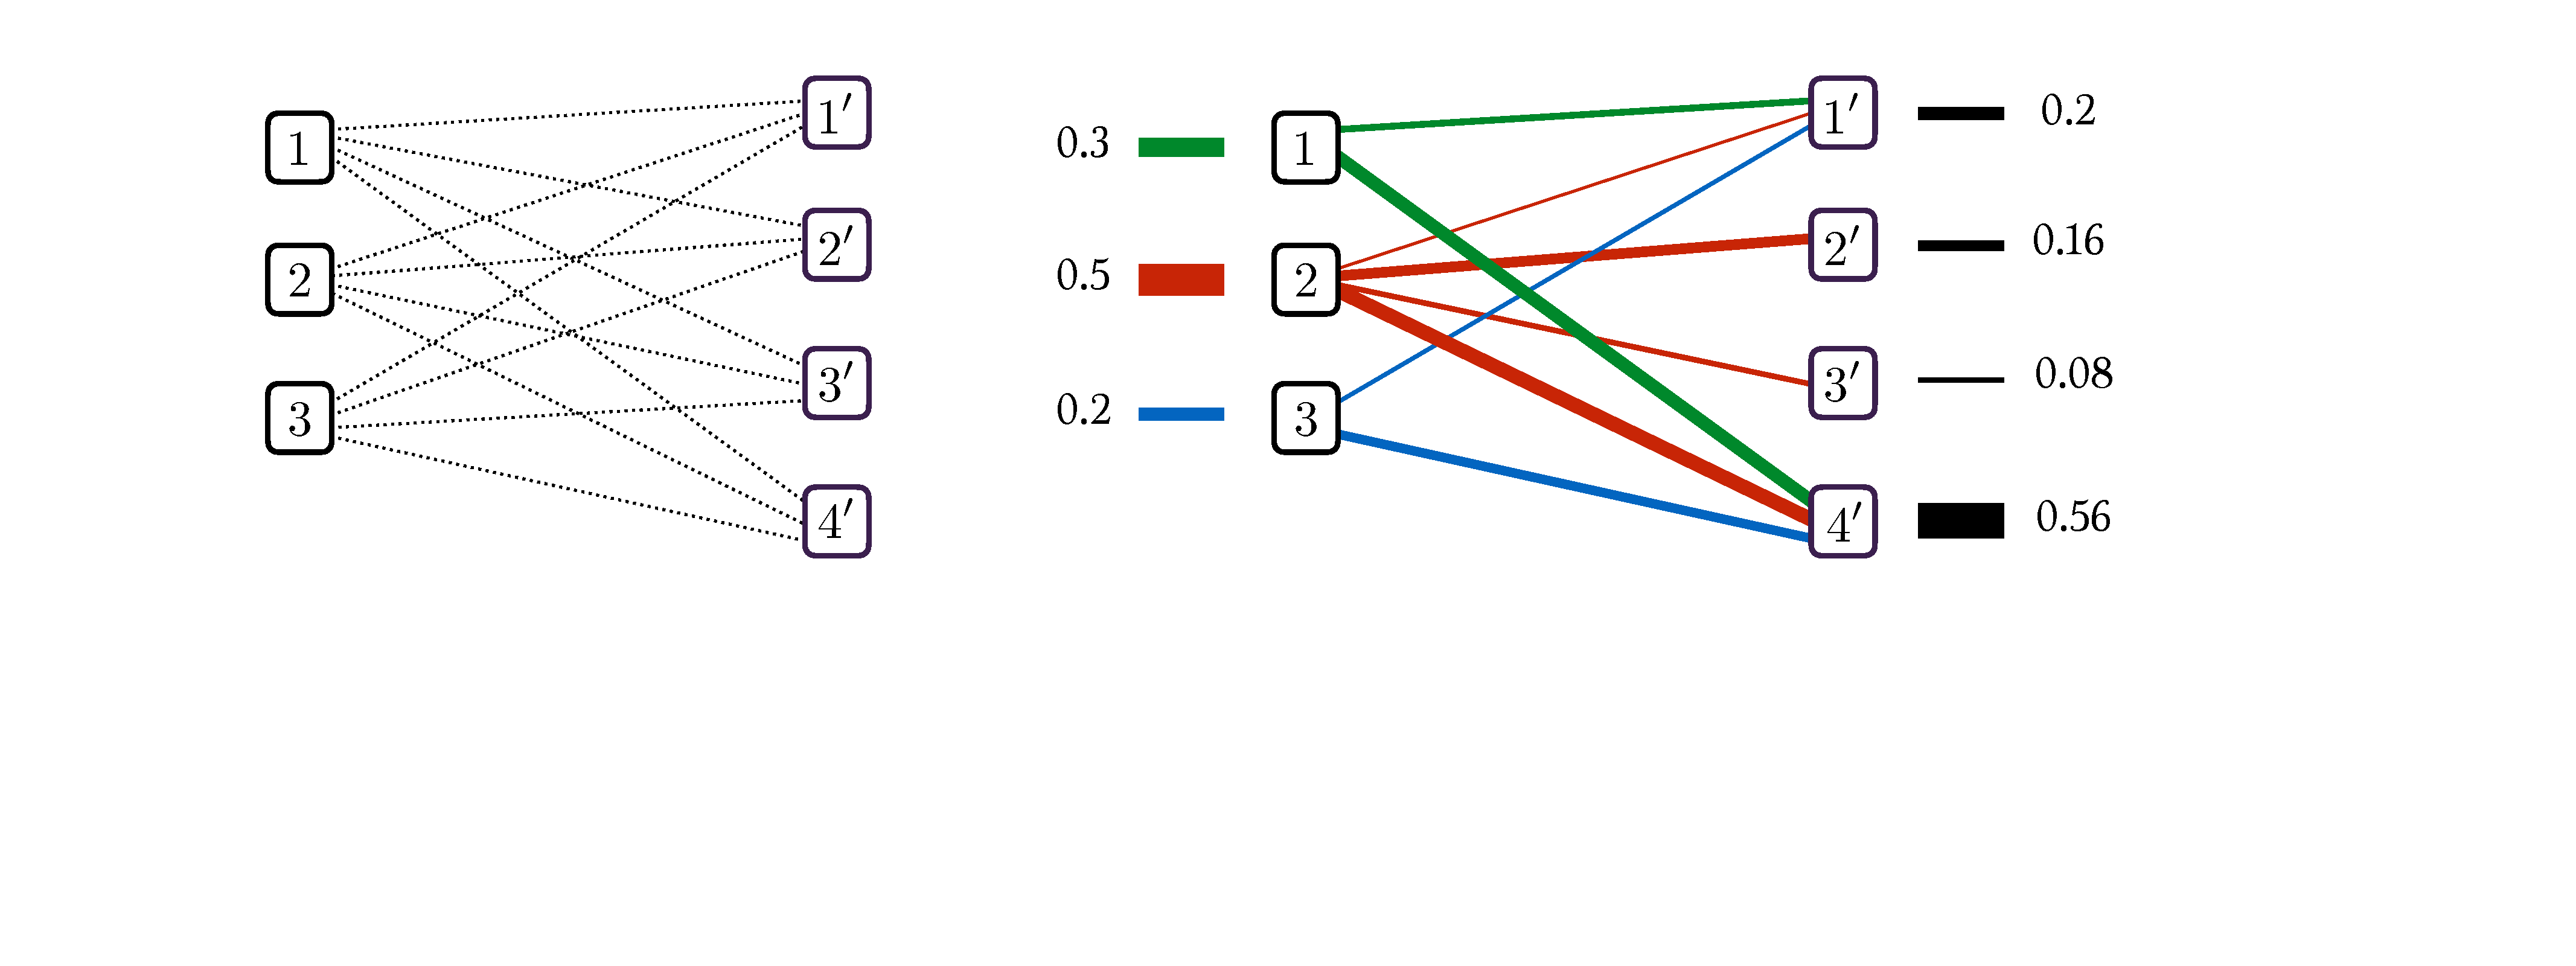
\includegraphics[width=\linewidth]{algo-basics-tree-solution/networksol}
\caption{\label{fig-simplex}
The optimal transport problem as a bipartite network flow problem. Here $n=3,m=4$. All coordinates of the source histogram, $\a$, are depicted as source nodes on the left labeled $1,2,3$, whereas all coordinates of the target histogram $\b$ are labeled as nodes $1',2',3',4'$. The graph is bipartite in the sense that all source nodes are connected to all target nodes, with no additional edges. To each edge $(i,j')$ is associated a cost $\C_{ij}$. A feasible flow is represented on the right. Proposition~\ref{prop-extremal} shows that this flow is not extremal since it has at least one cycle given by $((1,1'),(2,1'),(2,4'),(1,4'))$. 
}
\end{figure}


\begin{figure}[h!]
\centering
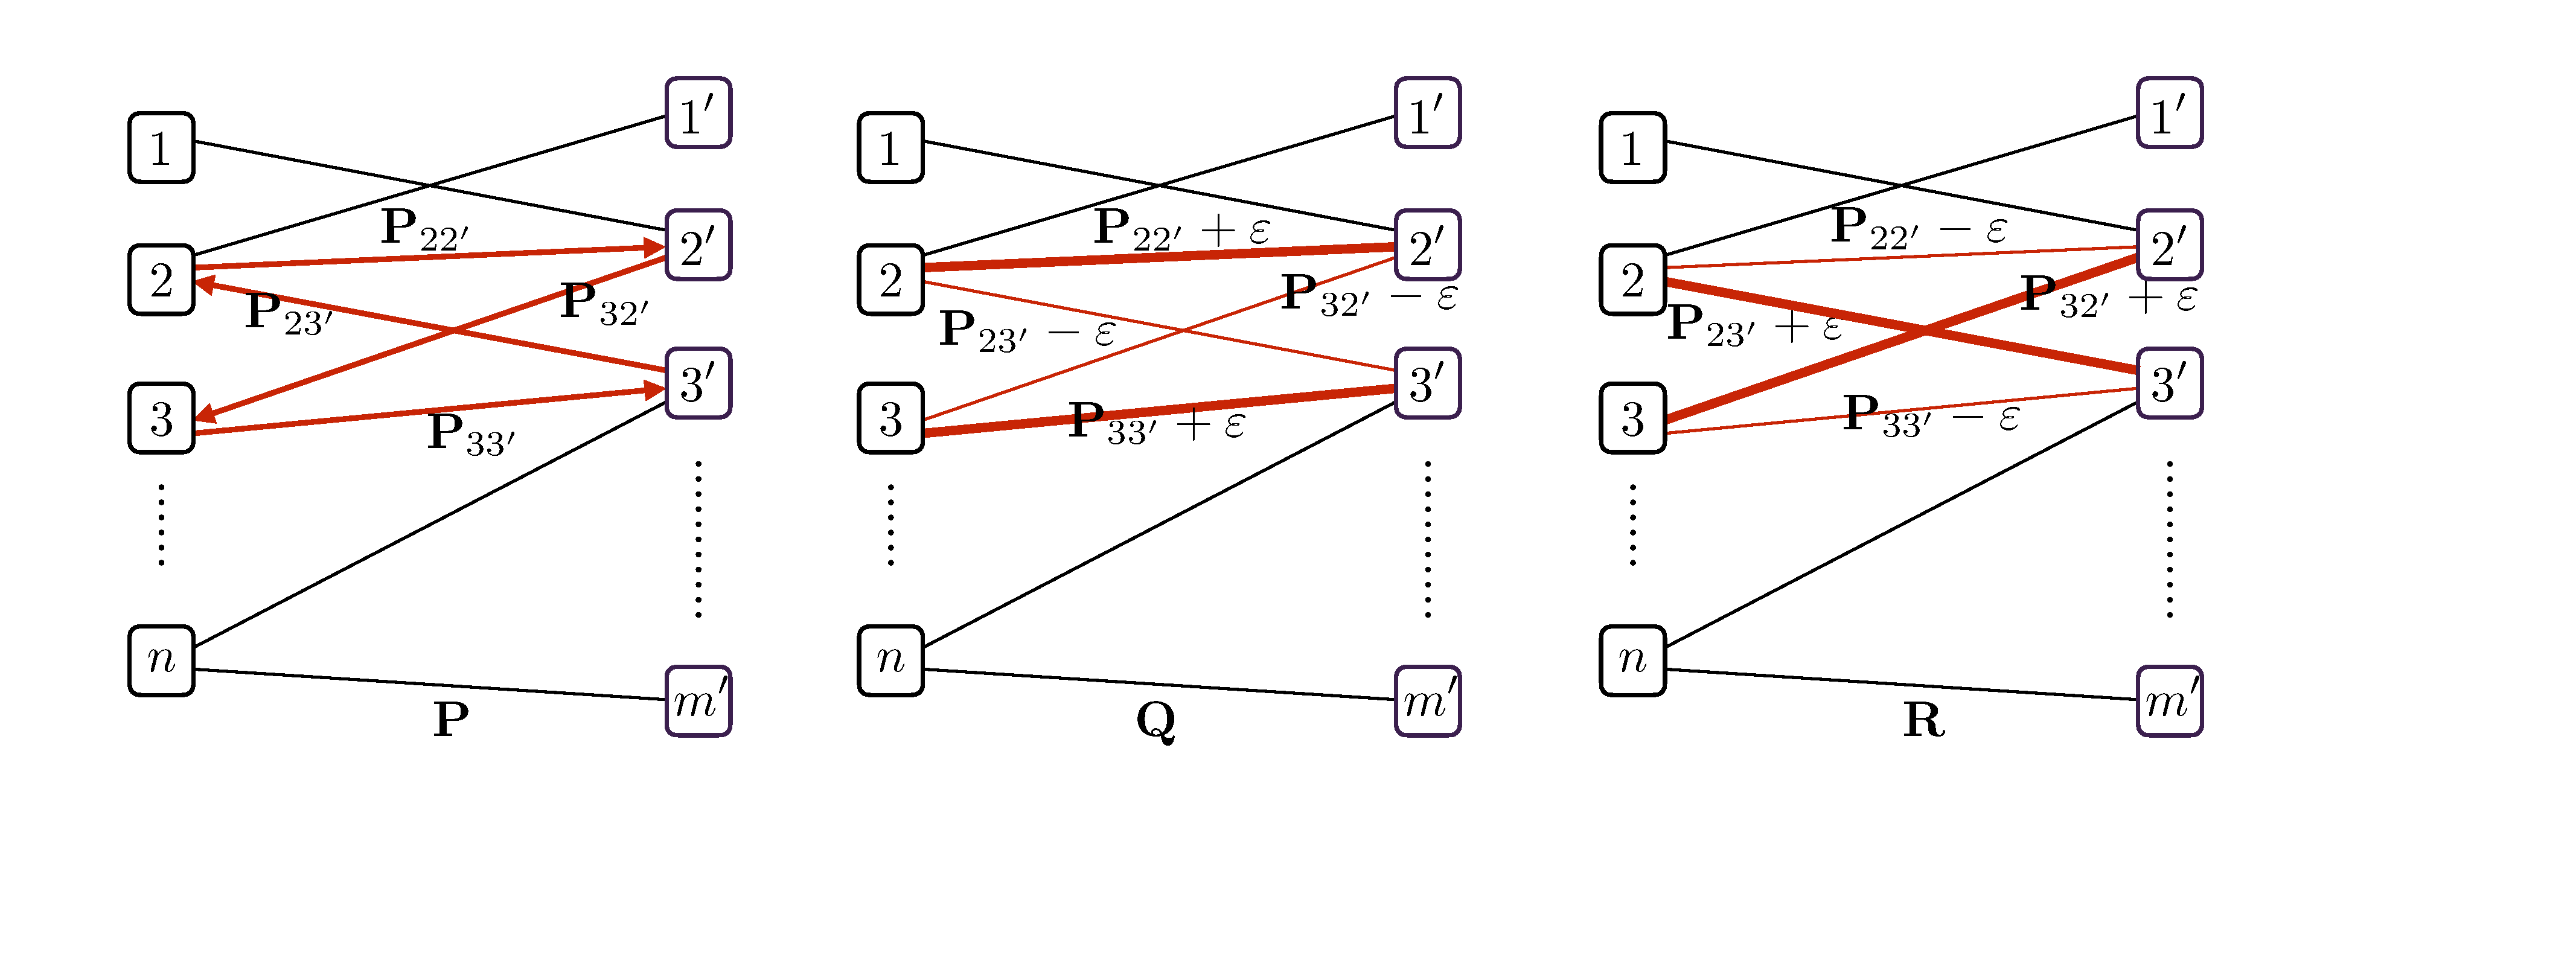
\includegraphics[width=\linewidth]{algo-basics-tree-solution/tree-sol2}
\caption{\label{fig-perturb}
A solution $\P$ with a cycle in the graph of its support can be perturbed to obtain two feasible solutions $\Q$ and $\RRd$ such that $\P$ is their average, therefore disproving that $\P$ is extremal. 
}
\end{figure}

\begin{prop}[Extremal solutions]\label{prop-extremal}
Let $\P$ be an extremal point of the polytope $\CouplingsD(\a,\b)$. Let $S(\P)\subset \alledges$ be the subset of edges $\{(i,j'), i\in\range{n}, j\in\range{m} \text{ such that } \P_{ij}>0\}$. Then the graph $G(\P)\eqdef (V\cup V',S(\P))$ has no cycles. In particular, $\P$ cannot have more than $n+m-1$ nonzero entries.
 \end{prop}
\begin{proof}
We proceed by contradiction. Suppose that $\P$ is an extremal point of the polytope $\CouplingsD(\a,\b)$ and that its corresponding set $S(\P)$ of edges, denoted $F$ for short, is such that the graph $G=(V\cup V',F)$ contains a cycle, namely there exists $k>1$ and a sequence of distinct indices $i_1,\dots,i_{k-1}\in\range{n}$ and $j_1,\dots,j_{k-1}\in\range{m}$ such that the set of edges $H$ given below forms a subset of $F$. $$H=\left\{(i_1,j_1'), (i_2,j_1'), (i_2,j_2'),\dots,(i_k,j_k'),(i_1,j_k')\right\}.$$ 
	We now construct two feasible matrices $\Q$ and $\RRd$ such that $\P=(\Q+\RRd)/2$. To do so, consider a \emph{directed} cycle $\bar{H}$ corresponding to $H$, namely the sequence of pairs $i_1\rightarrow j_1', j_1' \rightarrow i_2, i_2 \rightarrow j_2',\dots, i_k \rightarrow j_k' , j_k' \rightarrow i_1$, as well as the elementary amount of flow $\varepsilon < \min_{(i,j')\in F}\P_{ij}$.
	Consider a perturbation matrix $\E$ whose $(i,j)$ entry is equal to $\varepsilon$ if $i\rightarrow j' \in \bar{H}$, $-\varepsilon$ if $ j\rightarrow i'\in \bar{H}$, and zero otherwise. Define matrices $\Q=\P+\E$ and $\RRd=\P-\E$ as illustrated in Figure~\ref{fig-perturb}. Because $\varepsilon$ is small enough, all elements in $\Q$ and $\RRd$ are nonnegative. By construction, $\E$ has either lines (resp., columns) with all entries equal to $0$ or exactly one entry equal to $\varepsilon$ and another equal to $-\varepsilon$ for those indexed by $i_1,\dots,i_k$ (resp., $j_1,\dots,j_k$). Therefore, $\E$ is such that $\E\ones_{m}=\zeros_{n}$ and $\transp{\E}\ones_{n}=\zeros_{m}$, and we have that $\Q$ and $\RRd$ have the same marginals as $\P$, and are therefore feasible. Finally $\P=(\Q+\RRd)/2$ which, since $\Q,\RRd\ne \P$, contradicts the fact that $\P$ is an extremal point. Since a graph with $k$ nodes and no cycles cannot have more than $k-1$ edges, we conclude that $S(\P)$ cannot have more than $n+m-1$ edges, and therefore $\P$ cannot have more than $n+m-1$ nonzero entries. 
\end{proof}

\subsection{The North-West Corner Rule}\label{subsec-northwest}
The north-west (NW) corner rule is a heuristic that produces a vertex of the polytope $\CouplingsD(\a,\b)$ in up to $n+m$ operations. This heuristic can play a role in initializing any algorithm working on the primal, such as the network simplex outlined in the next section. 

The rule starts by giving the highest possible value to $\P_{1,1}$ by setting it to $\min(\a_1,\b_1)$. At each step, the entry $\P_{i,j}$ is chosen to saturate either the row constraint at $i$, the column constraint at $j$, or both if possible. The indices $i,j$ are then updated as follows: $i$ is incremented in the first case, $j$ is in the second, and both $i$ and $j$ are in the third case. The rule proceeds until $\P_{n,m}$ has received a value. 

Formally, the algorithm works as follows: $i$ and $j$ are initialized to $1$, $r\leftarrow\a_1,c\leftarrow \b_1$. While $i\leq n$ and $j\leq m$, set $t\leftarrow \min(r,c)$, $\P_{i,j}\leftarrow t$, $r\leftarrow r-t$, $c\leftarrow s-t$; if $r=0$ then increment $i$, and update $r\leftarrow\a_i$ if $i\leq n$; if $c=0$ then increment $j$, and update $c\leftarrow \b_j$ if $j\leq n$; repeat. Here is an example of this sequence assuming $\a=[0.2,0.5,0.3]$  and $\b=[0.5,0.1,0.4]$:
$$\begin{aligned}\begin{bmatrix} \bullet & 0 & 0 \\ 0 & 0 & 0 \\ 0& 0 & 0\end{bmatrix} &\rightarrow \begin{bmatrix} 0.2 & 0 & 0 \\ \bullet & 0 & 0 \\ 0& 0 & 0\end{bmatrix} &\rightarrow \begin{bmatrix} 0.2 & 0 & 0 \\ 0.3 & \bullet & 0 \\ 0& 0 & 0\end{bmatrix}\\ &\rightarrow \begin{bmatrix} 0.2 & 0 & 0 \\ 0.3 &0.1 &\bullet \\ 0& 0 & 0\end{bmatrix} &\rightarrow \begin{bmatrix} 0.2 & 0 & 0 \\ 0.3 &0.1 &0.1 \\ 0& 0 & \bullet\end{bmatrix} & \rightarrow \begin{bmatrix} 0.2 & 0 & 0 \\ 0.3 &0.1 &0.1 \\ 0& 0 & 0.3\end{bmatrix}\end{aligned}$$
We write $\NW(\a,\b)$ for the unique plan that can be obtained through this heuristic. 

Note that there is, however, a much larger number of NW corner solutions that can be obtained by permuting arbitrarily the order of $\a$ and $\b$ first, computing the corresponding NW corner table, and recovering a table of $\CouplingsD(\a,\b)$ by inverting again the order of columns and rows: setting $\sigma=(3,1,2),\sigma'=(3,2,1)$ gives $\a_\sigma=[0.3,0.2,0.5], \b_{\sigma'}=[0.4,0.1,0.5]$, and $\sigma^{-1}=(2,3,1),\sigma'=(3,2,1)$. Observe that
\begin{gather*}
\NW(\a_\sigma,\b_{\sigma'}) = \begin{bmatrix} 0.3 & 0 & 0 \\ 0.1 & 0.1 & 0 \\ 0& 0 & 0.5\end{bmatrix} \in \CouplingsD(\a_\sigma,\b_{\sigma'}),\\
\NW_{\sigma^{-1}\sigma'^{-1}}(\a_\sigma,\b_{\sigma'})= \begin{bmatrix} 0 & 0.1 & 0.1 \\ 0.5 & 0 & 0 \\ 0& 0 & 0.3\end{bmatrix}\in \CouplingsD(\a,\b).
\end{gather*}

Let $\mathcal{N}(\a,\b)$ be the set of all NW corner solutions that can be produced this way:
$$\mathcal{N}(\a,\b)\eqdef\{ \NW_{\sigma^{-1}\sigma'^{-1}}(r_\sigma,c_{\sigma'}), \sigma,\sigma'\in S_d\}.$$
All NW corner solutions have by construction up to $n+m-1$ nonzero elements. The NW corner rule produces a table which is by construction unique for $\a_\sigma$ and $\b_\sigma'$, but there is an exponential number of pairs or row/column permutations $(\sigma,\sigma')$ that may yield the same table~\citep[p. 2]{stougie2002polynomial}. $\mathcal{N}(\a,\b)$ forms a subset of (usually strictly included in) the set of extreme points of $\CouplingsD(\a,\b)$~\citep[Cor. 8.1.4]{brualdi2006combinatorial}.



\section{A Heuristic Description of the Network Simplex}\label{s-networksimplex}

Consider a feasible matrix $\P$ whose graph $G(\P)=(V\cup V',S(\P))$ has no cycles. $\P$ has therefore no more than $n+m-1$ nonzero entries and is a vertex of $\CouplingsD(\a,\b)$ by Proposition~\ref{prop-extremal}. 
%
Following Proposition~\ref{prop-primal-dual-optimality}, it is therefore sufficient to obtain a dual solution $(\fD,\gD)$ which is feasible (\ie $\C-\fD\oplus\gD$ has nonnegative entries) and complementary to $\P$ (pairs of indices $(i,j')$ in $S(\P)$ are such that $\C_{i,j}=\fD_i+\gD_j$), to prove that $\P$ is optimal. 
%
The network simplex relies on two simple principles: to each feasible primal solution $\P$ one can associate a complementary pair $(\fD,\gD)$. 
%
If that pair is feasible, then we have reached optimality. If not, one can consider a modification of $\P$ that remains feasible and whose complementary pair $(\fD,\gD)$ is modified so that it becomes closer to feasibility.

\subsection{Obtaining a Dual Pair Complementary to $\P$}\label{subsec-obtaining}
The simplex proceeds by associating first to any extremal solution $\P$ a pair of $(\fD,\gD)$ complementary dual variables. This is simply carried out by finding two vectors $\fD$ and $\gD$ such that for any $(i,j')$ in $S(\P)$, $\fD_i+\gD_j$ is equal to $\C_{i,j}$. Note that this, in itself, does not guarantee that $(\fD,\gD)$ is feasible.

\begin{figure}[h!]
	\centering
	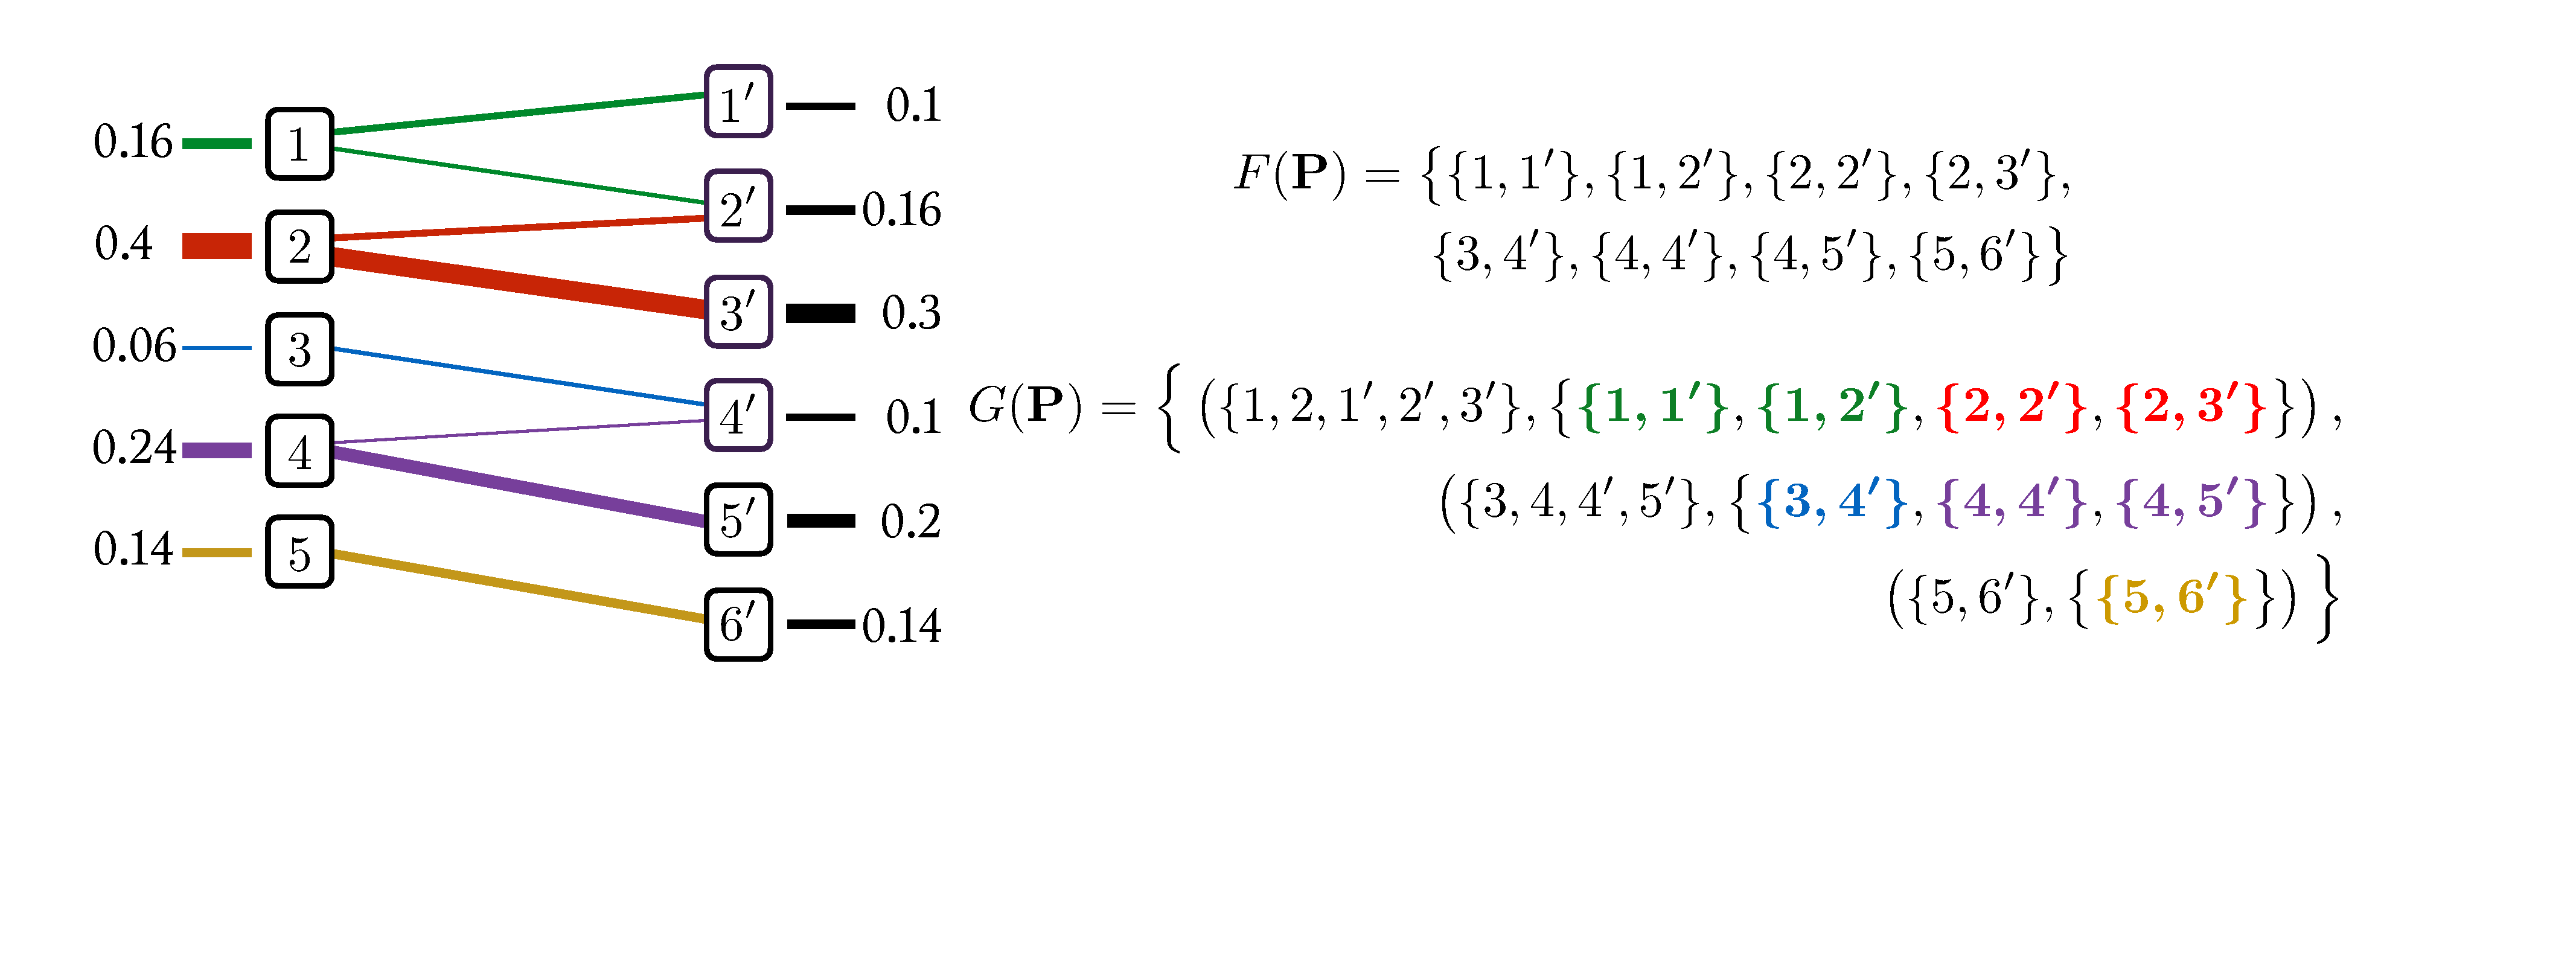
\includegraphics[width=\linewidth]{algo-basics-tree-solution/f_of_P}
	\caption{\label{fig-f_of_P}
	A feasible transport $\P$ and its corresponding set of edges $S(\P)$ and graph $G(\P)$. As can be seen, the graph $G(\P)=(\{1,\dots,5,1',\dots,6'\},S(\P))$ is a forest, meaning that it can be expressed as the union of tree graphs, three in this case.}
\end{figure}


Let $s$ be the cardinality of $S(\P)$. Because $\P$ is extremal, $s\leq n+m-1$. Because $G(\P)$ has no cycles, $G(\P)$ is either a tree or a forest (a union of trees), as illustrated in Figure~\ref{fig-f_of_P}. Aiming for a pair $(\fD,\gD)$ that is complementary to $\P$, we consider the following set of $s$ linear equality constraints on $n+m$ variables:
\begin{equation}\label{eq-dual-variables}
	\begin{array}{ccc}
\fD_{i_1}+\gD_{j_1}&=&\C_{i_1,j_1}\\
\fD_{i_2}+\gD_{j_1}&=&\C_{i_2,j_1}\\
\vdots & = & \vdots\\
\fD_{i_s}+\gD_{j_s}&=&\C_{i_s,j_s},\\
\end{array}
\end{equation}
where the elements of $S(\P)$ are enumerated as $(i_1,j_1'),\dots,(i_s,j_s')$.

Since $s\leq n+m-1 < n+m$, the linear system~\eqref{eq-dual-variables} above is always undetermined. This degeneracy can be interpreted in part because the parameterization of $\CouplingsD(\a,\b)$ with $n+m$ constraints results in $n+m$ dual variables. A more careful formulation, outlined in Remark~\ref{rem-transportation-polytope}, would have resulted in an equivalent formulation with only $n+m-1$ constraints and therefore $n+m-1$ dual variables. However, $s$ can also be strictly smaller than $n+m-1$: This happens when $G(\P)$ is the disjoint union of two or more trees. For instance, there are $5+6=11$ dual variables (one for each node) in Figure~\ref{fig-f_of_P}, but only $8$ edges among these $11$ nodes, namely $8$ linear equations to define $(\fD,\gD)$. Therefore, there will be as many undetermined dual variables under that setting as there will be connected components in $G(\P)$. 

Consider a tree among those listed in $G(\P)$. Suppose that tree has $k$ nodes $i_1,\dots,i_k$ among source nodes and $l$ nodes $j_1',\dots,j_{l}'$ among target nodes, resulting in $r\eqdef k+l$, and $r-1$ edges, corresponding to $k$ variables in $\fD$ and $l$ variables in $\gD$, linked with $r-1$ linear equations. To lift an indetermination, we can choose arbitrarily a root node in that tree and assign the value $0$ to its corresponding dual variable. From there, we can traverse the tree using a breadth-first or depth-first search to obtain a sequence of simple variable assignments that determines the values of all other dual variables in that tree, as illustrated in Figure~\ref{fig-tree-linear-solve}. That procedure can then be repeated for all trees in the graph of $\P$ to obtain a pair of dual variables $(\fD,\gD)$ that is complementary to $\P$.

\begin{figure}[h!]
	\centering
	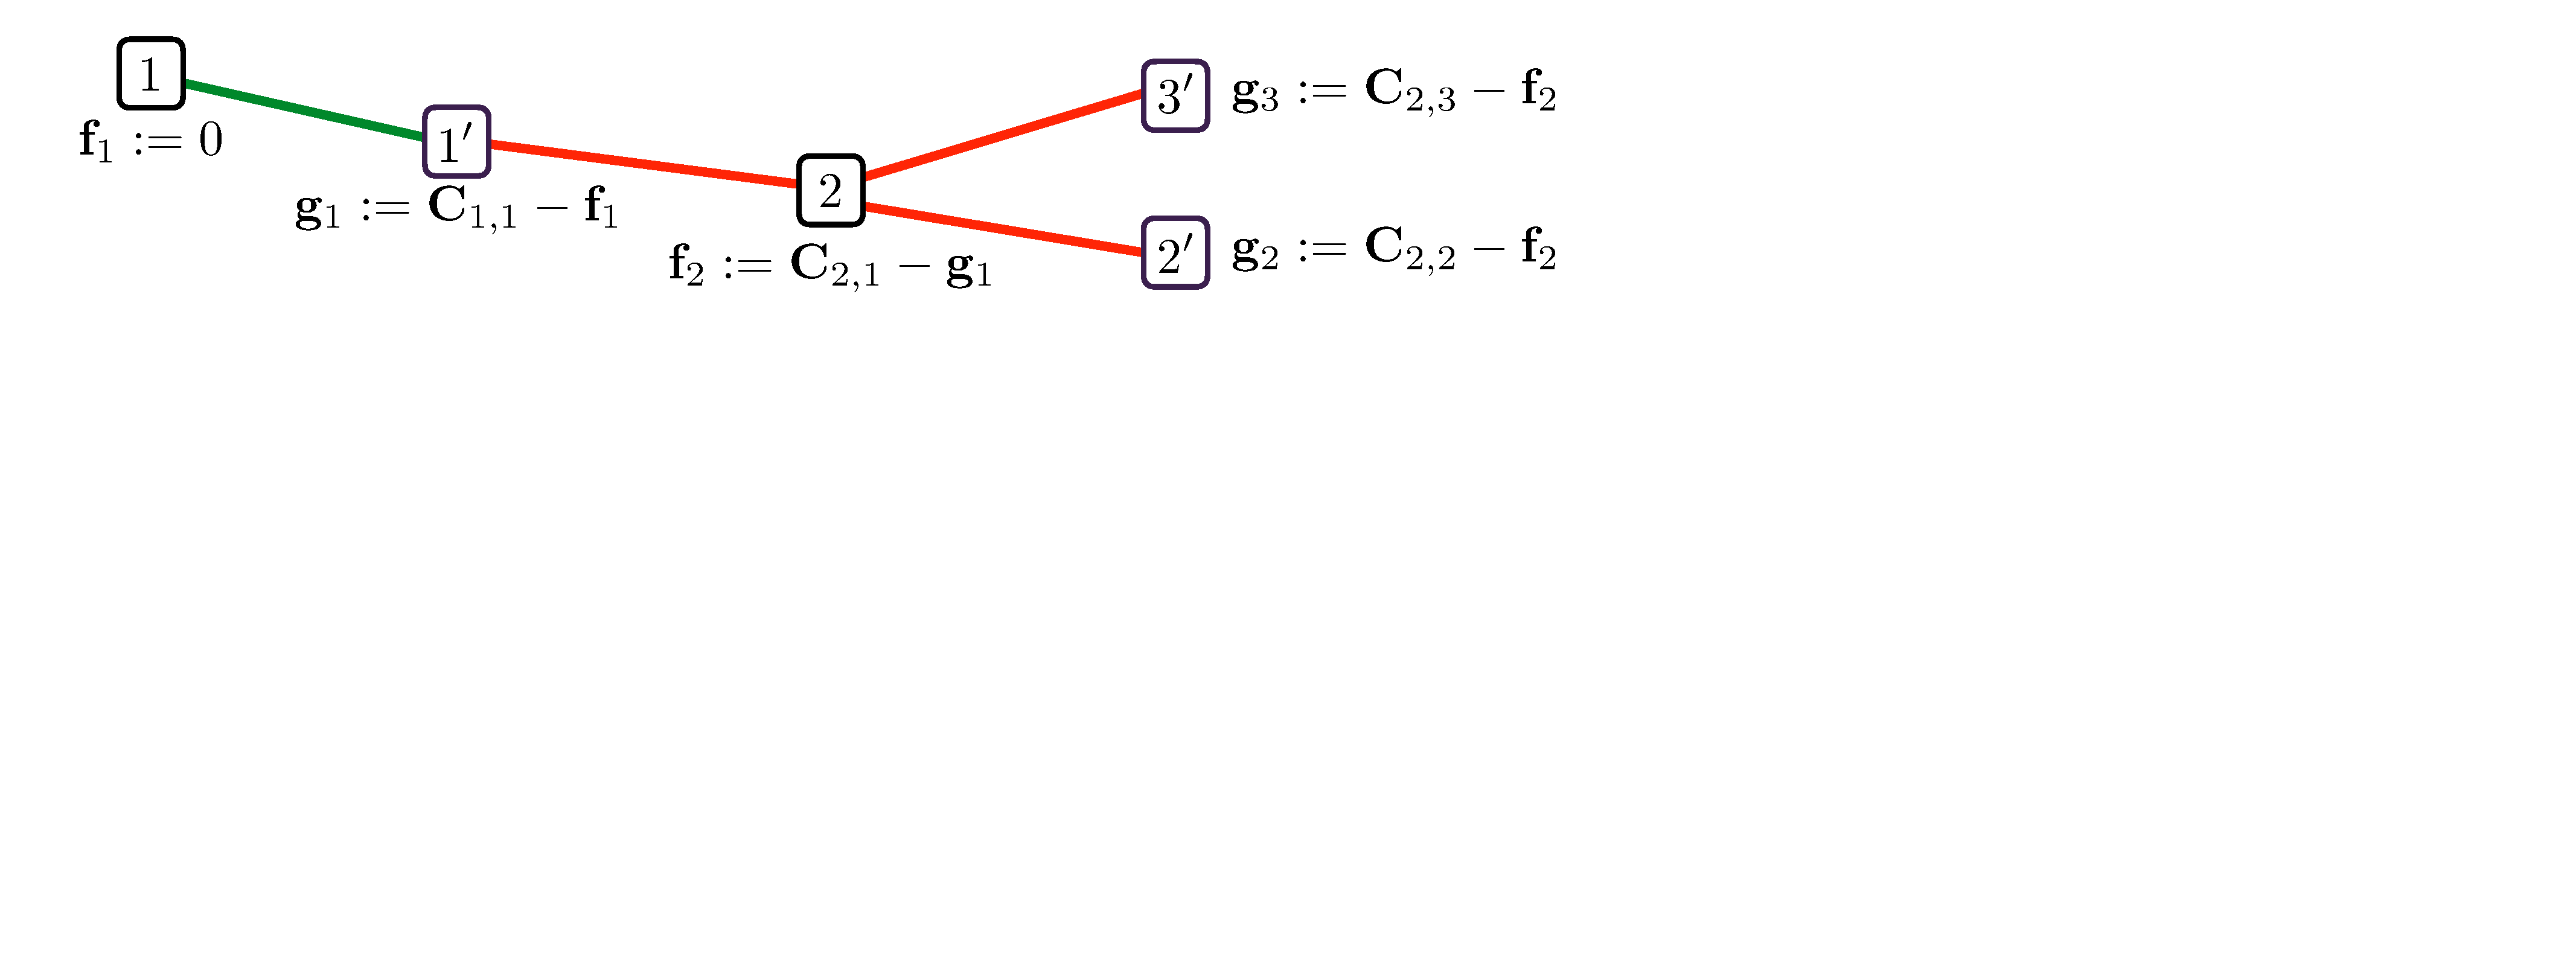
\includegraphics[width=\linewidth]{algo-basics-tree-solution/tree-linear-solve}
	\caption{\label{fig-tree-linear-solve}
 The five dual variables $\fD_1,\fD_2,\gD_1,\gD_2,\gD_3$ corresponding to the five nodes appearing in the first tree of the graph $G(\P)$ illustrated in Figure \ref{fig-f_of_P} are linked through four linear equations that involve corresponding entries in the cost matrix $\C$. Because that system is degenerate, we choose a root in that tree (node 1 in this example) and set its corresponding variable to $0$ and proceed then by traversing the tree (either breadth-first or depth-first) from the root to obtain iteratively the values of the four remaining dual variables.}
\end{figure}

\subsection{Network Simplex Update}
The dual pair $(\fD,\gD)$ obtained previously might be feasible, in the sense that for all $i,j$ we have $\fD_i+\gD_j\leq \C_{i,j}$, in which case we have reached the optimum by Proposition~\ref{prop-primal-dual-optimality}. When that is not the case, namely when there exists $i,j$ such that $\fD_i+\gD_j> \C_{i,j}$, the network simplex algorithm kicks in. We first initialize a graph $G$ to be equal to the graph $G(\P)$ corresponding to the feasible solution $\P$ and add the violating edge $(i,j')$ to $G$. Two cases can then arise:
\begin{enumerate}[label={(\alph*)}]
	\item $G$ is (still) a forest, which can happen if $(i,j')$ links two existing subtrees. The approach outlined in~\S\ref{subsec-obtaining} can be used on graph $G$ to recover a new complementary dual vector $(\fD,\gD)$. Note that this addition simply removes an indetermination among the $n+m$ dual variables and does not result in any change in the primal variable $\P$. That update is usually called degenerate in the sense that $(i,j')$ has now entered graph $G$ although $\P_{i,j}$ remains $0$. $G(\P)$ is, however, contained in $G$.
	
	\item $G$ now has a cycle. In that case, we need to remove an edge in $G$ to ensure that $G$ is still a forest, yet also modify $\P$ so that $\P$ is feasible and $G(\P)$ remains included in $G$. These operations can all be carried out by increasing the value of $\P_{i,j}$ and modifying the other entries of $\P$ appearing in the detected cycle, in a manner very similar to the one we used to prove Proposition~\ref{prop-extremal}. To be more precise, let us write that cycle $(i_1,j_1'), (j_1',i_2), (i_2,j_2'),\dots, (i_l,j_l'),(j_l',i_{l+1})$ with the convention that $i_1=i_{l+1}=i$ to ensure that the path is a cycle that starts and ends at $i$, whereas $j_1=j$, to highlight the fact that the cycle starts with the added edge $\{i,j\}$, going in the right direction. Increase now the flow of all ``positive'' edges $(i_k,j_k')$ (for $k\leq l$), and decrease that of ``negative'' edges $(j_k',i_{k+1})$ (for $k\leq l$), to obtain an updated primal solution $\tilde{\P}$, equal to $\P$ for all but the following entries:
$$\forall k\leq l,\quad \tilde{\P}_{i_k,j_k}:= \P_{i_k,j_k}+\theta;\quad \tilde{\P}_{i_{k+1},j_k}:= \P_{i_{k+1},j_k}-\theta.$$
Here, $\theta$ is the largest possible increase at index $i,j$ using that cycle. The value of $\theta$ is controlled by the smallest flow negatively impacted by the cycle, namely $\min_{k} \P_{i_{k+1},j_k}$. That update is illustrated in Figure~\ref{fig-simplex-update}. Let $k^\star$ be an index that achieves that minimum. We then close the update by removing $(i_{k^\star+1},j_{k^\star})$ from $G$, to compute new dual variables $(\fD,\gD)$ using the approach outlined in~\S\ref{subsec-obtaining}.  
\end{enumerate}
	
\subsection{Improvement of the Primal Solution} Although this was not necessarily our initial motivation, one can show that the manipulation above can only improve the cost of $\P$. If the added edge has not created a cycle, case {(a)} above, the primal solution remains unchanged. When a cycle is created, case {(b)}, $\P$ is updated to $\tilde{\P}$, and the following equality holds:
\eq{
\dotp{\tilde{\P}}{\C}-\dotp{\P}{\C}= \theta \left(\;\sum_{k=1}^{l} \C_{i_k,j_k} - \sum_{k=1}^{l}\C_{i_{k+1},j_k}\right).
}
We now use the dual vectors $(\fD,\gD)$ computed at the end of the previous iteration. They are such that $\f_{i_k}+\g_{i_k}=\C_{i_k,j_k}$ and $\f_{i_{k+1}}+\g_{i_k}=\C_{i_{k+1},j_k}$ for \emph{all} edges initially in $G$, resulting in the identity
\eq{
\begin{aligned}\sum_{k=1}^{l} \C_{i_k,j_k} - \sum_{k=1}^{l}\C_{i_{k+1},j_k} &= \C_{i,j} + \sum_{k=2}^{l} \fD_{i_k}+\gD_{j_k} - \sum_{k=1}^{l} \fD_{i_{k+1}}+\gD_{j_k}\\
	&= \C_{i,j} - (\fD_{i} +\gD_{j}).
\end{aligned}
}
That term is, by definition, negative, since $i,j$ were chosen because $C_{i,j} < \fD_{i} -\gD_{j}$. Therefore, if $\theta>0$, we have that \eq{\dotp{\tilde{\P}}{\C}=\dotp{\P}{\C}+\theta\left(\C_{i,j}-(\fD_{i} -\fD_{g})\right)<\dotp{\P}{\C}.} 
If $\theta=0$, which can happen if $G$ and $G(\P)$ differ, the graph $G$ is simply changed, but $\P$ is not.


\begin{figure}[h!]
	\centering
	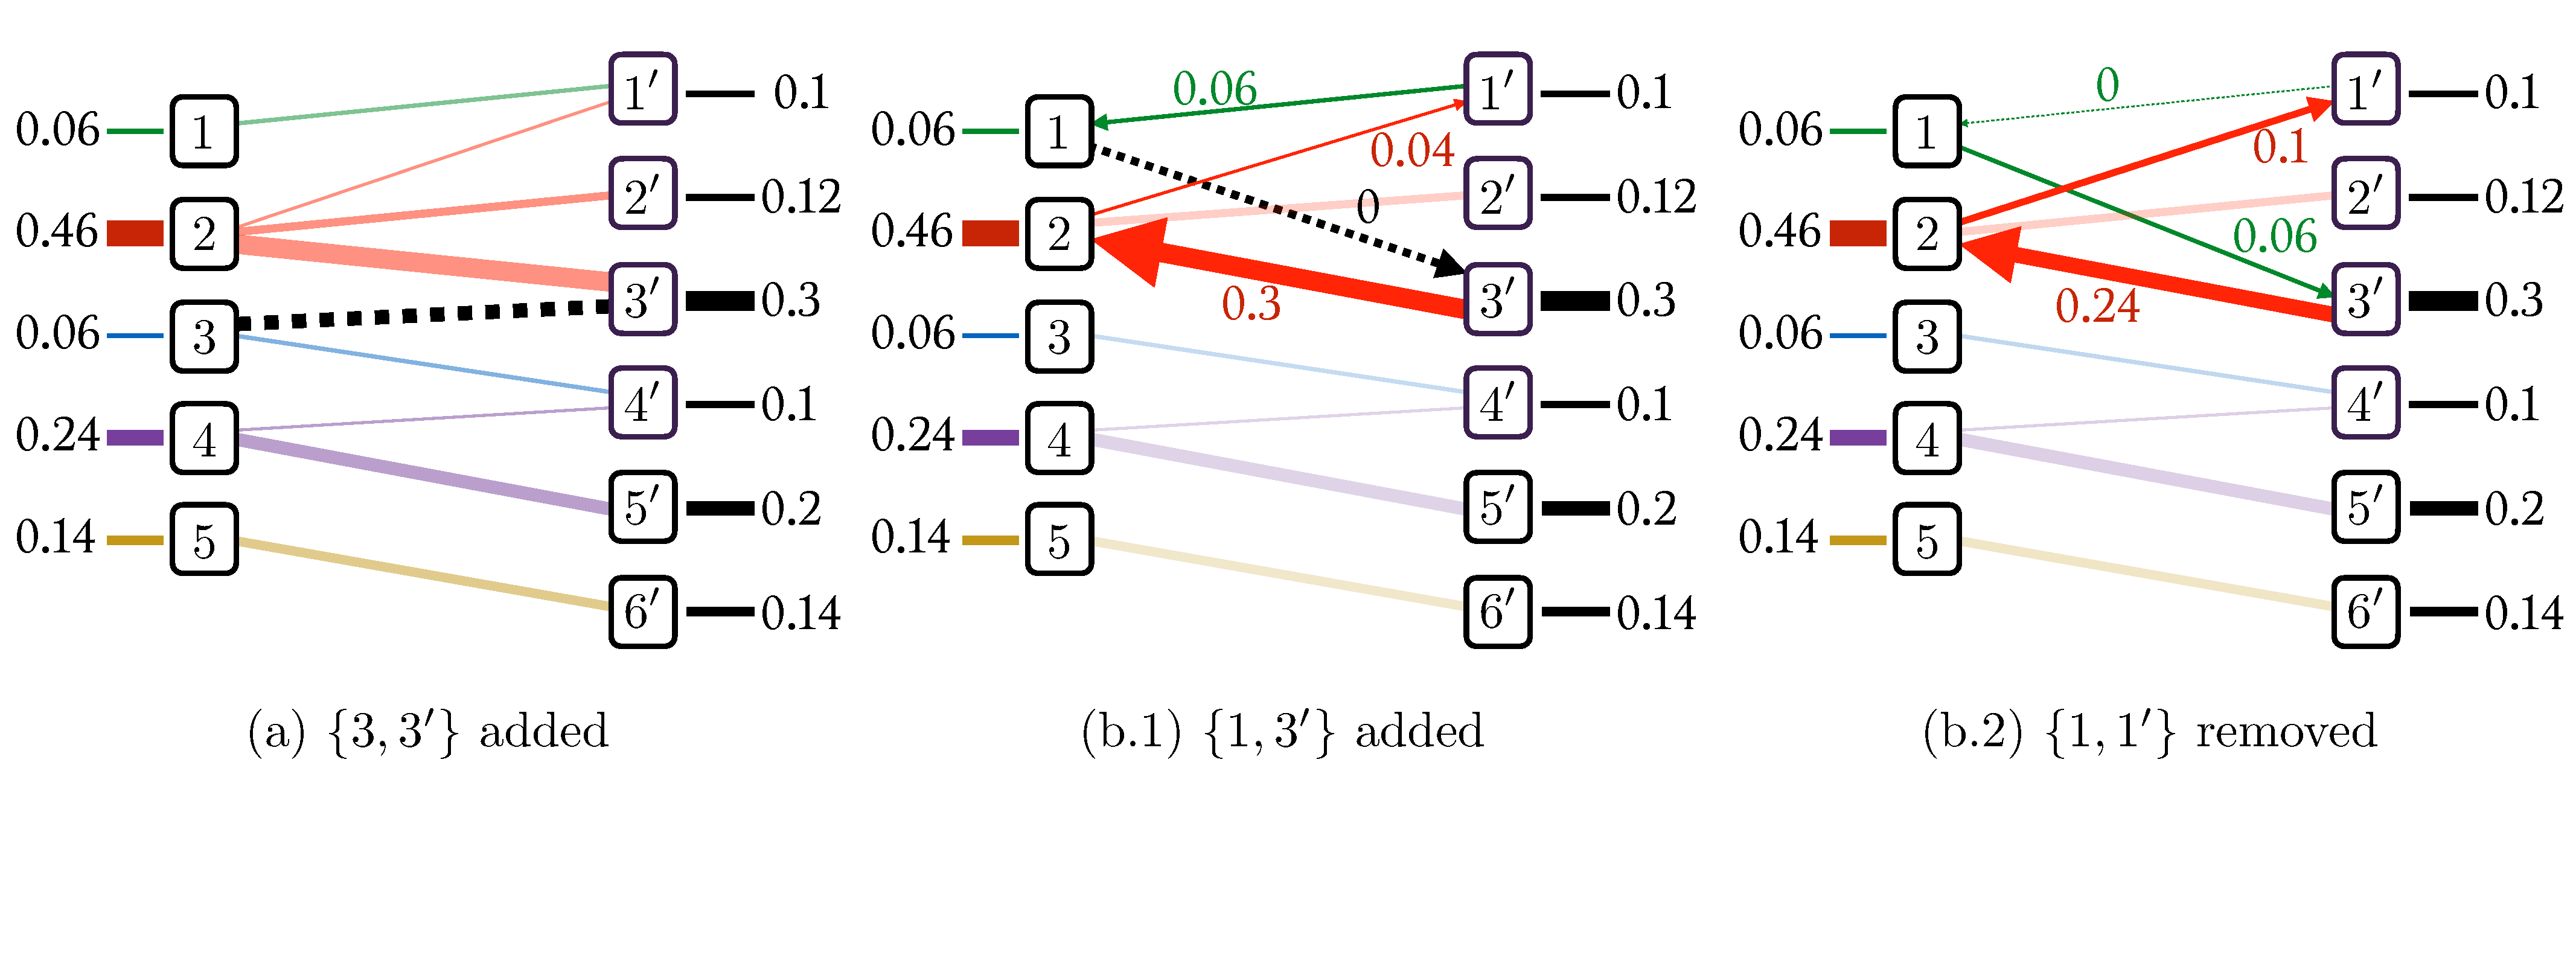
\includegraphics[width=\linewidth]{algo-basics-tree-solution/simplex-update}
	\caption{\label{fig-simplex-update}
Adding an edge $\{i,j\}$ to the graph $G(\P)$ can result in either (a) the graph remains a forest after this addition, in which case $\fD,\gD$ can be recomputed following the approach outlined in~\S\ref{subsec-obtaining}; (b.1) the addition of that edge creates a cycle, from which we can define a directed path; (b.2) the path can be used to increase the value of $\P_{i,j}$ and propagate that change along the cycle to maintain the flow feasibility constraints, until the flow of one of the edges that is negatively impacted by the cycle is decreased to $0$. This removes the cycle and updates $\P$.}
\end{figure}

The network simplex algorithm can therefore be summarized as follows: Initialize the algorithm with an extremal solution $\P$, given for instance by the NW corner rule as covered in~\S\ref{subsec-northwest}. Initialize the graph $G$ with $G(\P)$. Compute a pair of dual variables $(\fD,\gD)$ that are complementary to $\P$ using the linear system solve using the tree structure(s) in $G$ as described in~\S\ref{subsec-obtaining}. {(i)} Look for a violating pair of indices to the constraint $\C- \fD\oplus \gD\geq 0$; if none, $\P$ is optimal and stop. If there is a violating pair $(i,j')$, {(ii)} add the edge $(i,j')$ to $G$. If $G$ still has no cycles, update $(\fD,\gD)$ accordingly; if there is a cycle, direct it making sure $(i,j')$ is labeled as positive, and remove a negative edge in that cycle with the smallest flow value, updating $\P,G$ as illustrated in Figure~\ref{fig-simplex-update}, then build a complementary pair $\fD,\gD$ accordingly; return to {(i)}. Some of the operations above require graph operations (cycle detection, tree traversals) which can be implemented efficiently in this context, as described in (\cite[\S5]{bertsekas1998network}).

\citet{Orlin1997} was the first to prove the polynomial time complexity of the network simplex.~\citet{Tarjan1997} provided shortly after an improved bound in $O\left(\,(n+m)nm \log(n+m)\log\left((n+m)\|\C\|_\infty\right)\,\right)$ which relies on more efficient data structures to help select pivoting edges.



%\paragraph{Improvement on $\P$.} Introducing a new edge $\{i,j\}$ in $G(\P)$ only because that pair violated the complementary requirement, namely because $\fD_i+\gD_j$ is strictly larger that $\C_{i,j}$, may seem like a valid approach to get closer to the goal of obtaining a feasible pair $(\fD,\gD)$ but it does not necessarily explain why this would result in a better solution $\P$ at all. 

\section{Dual Ascent Methods}\label{s-dual-ascent}

Dual ascent methods precede the network simplex by a few decades, since they can be traced back to work by~\citet{borchardt1865investigando} and later K\"onig and Egerv\'ary, as recounted by~\citet{Kuhn1955}. The Hungarian algorithm is the best known algorithm in that family, and it can work only in the particular case when $\a$ and $\b$ are equal and are both uniform, namely $\a=\b=\ones_n/n$. We provide in what follows a concise description of the more general family of dual ascent methods. This requires the knowledge of the maximum flow problem (\cite[\S7.5]{bertsimas1997introduction}). By contrast to the network simplex, presented above in the primal, dual ascent methods maintain at each iteration dual feasible solutions whose objective is progressively improved by adding a sparse vector to $\fD$ and $\gD$. Our presentation is mostly derived from that of (\cite[\S7.7]{bertsimas1997introduction}) and starts with the following definition.

\begin{defn} For $S\subset\range{n},S'\subset\range{m}'\eqdef \{1',\dots,m'\}$ we write $\ones_S$ for the vector in $\RR^n$ of zeros except for ones at the indices enumerated in $S$, and likewise for the vector $\ones_{S'}$ in $\RR^m$ with indices in $S'$. 
\end{defn}	

In what follows, $(\fD,\gD)$ is a feasible dual pair in $\PotentialsD(\C)$. Recall that this simply means that for all pairs $(i,j')\in\range{n}\times\range{m}'$, $\fD_i+\gD_j\leq\C_{ij}$. We say that $(i,j')$ is a \emph{balanced} pair (or edge) if $\fD_i+\gD_j=\C_{ij}$ and \emph{inactive} otherwise, namely if $\fD_i+\gD_j<\C_{ij}$. With this convention, we start with a simple result describing how a feasible dual pair $(\fD,\gD)$ can be perturbed using sparse vectors indexed by sets $S$ and $S'$ and still remain feasible.
	
\begin{prop}\label{prop-feasibility-dual-pair}
$(\tilde{\fD},\tilde{\gD})\eqdef(\fD,\gD)+\varepsilon(\ones_S,-\ones_{S'})$ is dual feasible for a small enough $\varepsilon>0$ if for all $i\in S$, the fact that $(i,j')$ is balanced implies that $j'\in S'$.
\end{prop}
\begin{proof}
For any $i\in S$, consider the set $\mathcal{I}_{i}$ of all $j'\in\range{m}'$ such that $(i,j')$ is inactive, namely such that $\fD_i+\gD_j<\C_{ij}$. Define $\varepsilon_i \eqdef \min_{j\in I_{i}} \C_{i,j}-\fD_i-\gD_j$, the smallest margin by which $\fD_i$ can be increased without violating the constraints corresponding to $j'\in \mathcal{I}_i$. Indeed, one has that if $\varepsilon\leq \varepsilon_i$ then $\tilde{\fD}_i+\tilde{\gD}_j<\C_{i,j}$ for any $j'\in \mathcal{I}_i$. Consider now the set $\mathcal{B}_i$ of balanced edges associated with $i$. Note that $\mathcal{B}_i=\range{m}'\setminus \mathcal{I}_i$. The assumption above is that $j'\in\mathcal{B}_i\Rightarrow j'\in S'$. Therefore, one has that for $j'\in\mathcal{B}_i$, $\tilde{\fD}_i+\tilde{\gD}_j=\fD_i+\gD_j=\C_{i,j}$. As a consequence, the inequality $\tilde{\fD}_i+\tilde{\gD}_j\leq \C_{i,j}$ is ensured for any $j\in \range{m}'$. Choosing now an increase $\varepsilon$ smaller than the smallest possible allowed, namely $\min_{i\in S} \varepsilon_i$, we recover that $(\tilde{\fD},\tilde{\gD})$ is dual feasible.
\end{proof}

The main motivation behind the iteration of the network simplex presented in \S\ref{subsec-obtaining} is to obtain, starting from a feasible primal solution $\P$, a complementary feasible dual pair $(\fD,\gD)$. To reach that goal, $\P$ is progressively modified such that its complementary dual pair reaches dual feasibility. A symmetric approach, starting from a feasible dual variable to obtain a feasible primal $\P$, motivates dual ascent methods. The proposition below is the main engine of dual ascent methods in the sense that it guarantees (constructively) the existence of an ascent direction for $(\fD,\gD)$ that maintains feasibility. That direction is built, similarly to the network simplex, by designing a candidate primal solution $\P$ whose infeasibility guides an update for $(\fD,\gD)$.

\begin{prop}\label{prop-dual-ascent-dir} Either $(\fD,\gD)$ is optimal for Problem~\eqref{eq-dual-discrete-split} or there exists $S\subset\range{n},S'\subset\range{m}'$ such that $(\tilde{\fD},\tilde{\gD})\eqdef(\fD,\gD)+\varepsilon(\ones_S,-\ones_{S'})$ is feasible for a small enough $\varepsilon>0$ and has a strictly better objective.
\end{prop}
\begin{proof}
We consider first a complementary primal variable $\P$ to $(\fD,\gD)$. To that effect, let $\mathcal{B}$ be the set of balanced edges, namely all pairs $(i,j')\in\range{n}\times\range{m}'$ such that $\fD_i+\gD_j=\C_{i,j}$, and form the bipartite graph whose vertices $\{1,\dots,n,1',\dots,m'\}$ are linked with edges in $\mathcal{B}$ only, complemented by a source node $s$ connected with \emph{capacitated} edges to all nodes $i\in\range{n}$ with respective capacities $\a_i$, and a terminal node $t$ also connected to all nodes $j'\in\range{m}'$ with edges of respective capacities $\b_j$, as seen in Figure~\ref{fig-dualascent}. The Ford--Fulkerson algorithm (\cite[p. 305]{bertsimas1997introduction}) can be used to compute a maximal flow $\mathbf{F}$ on that network, namely a family of $n+m+|\mathcal{B}|$ nonnegative values indexed by $(i,j')\in \mathcal{B}$ as $f_{si}\leq \a_i, f_{ij'}, f_{j't}\leq\b_j$ that obey flow constraints and such that $\sum_i f_{si}$ is maximal. If the throughput of that flow $\mathbf{F}$ is equal to $1$, then a feasible primal solution $\P$, complementary to $\fD,\gD$ by construction, can be extracted from $\mathbf{F}$ by defining $\P_{i,j}=f_{ij'}$ for $(i,j')\in \mathcal{B}$ and zero elsewhere, resulting in the optimality of $(\fD,\gD)$ and $\P$ by Proposition~\ref{prop-primal-dual-optimality}. If the throughput of $\mathbf{F}$ is strictly smaller than $1$, the labeling algorithm proceeds by labeling (identifying) those nodes reached iteratively from $s$ for which $\mathbf{F}$ does not saturate capacity constraints, as well as those nodes that contribute flow to any of the labeled nodes. Labeled nodes are stored in a nonempty set $Q$, which does not contain the terminal node $t$ per optimality of $\mathbf{F}$ (see \citealt[p. 308]{bertsimas1997introduction}, for a rigorous presentation of the algorithm). $Q$ can be split into two sets $S=Q\cap\range{n}$ and $S'=Q\cap\range{m}'$. Because we have assumed that the total throughput is strictly smaller than $1$, $S\ne\emptyset$. Note first that if $i\in S$ and $(i,j)$ is balanced, then $j'$ is necessarily in $S'$. Indeed, since all edges $(i,j')$ have infinite capacity by construction, the labeling algorithm will necessarily reach $j'$ if it includes $i$ in $S$. By Proposition~\ref{prop-feasibility-dual-pair}, there exists thus a small enough $\varepsilon$ to ensure the feasibility of $\tilde{\fD},\tilde{\gD}$. One still needs to prove that $\transp{\ones_S}{\a}-\transp{\ones_{S'}}{\b}>0$ to ensure that $(\tilde{\fD},\tilde{\gD})$ has a better objective than $(\fD,\gD)$. Let $\bar{S}=\range{n}\setminus S$ and $\bar{S'}=\range{m}'\setminus S'$ and define
$$A = \sum_{i\in S} f_{si}, \quad B = \sum_{i\in \bar{S}} f_{si}, \quad C = \sum_{j'\in S'} f_{j't}, \quad D = \sum_{j'\in \bar{S'}} f_{j't}.$$
The total maximal flow starts from $s$ and is therefore equal to $A+B$, but also arrives at $t$ and is therefore equal to $C+D$. Flow conservation constraints also impose that the very same flow is equal to $B+C$, therefore $A=C$. On the other hand, by definition of the labeling algorithm, we have for all $i$ in $S$ that $f_{si}<\a_i$, whereas $f_{j't}=\b_j$ for $j'\in \bar{S}'$ because $t$ cannot be in $S'$ by optimality of the considered flow. We therefore have $A<\transp{\ones_S}\a$ and $C=\transp{\ones_S'}\b$. Therefore $\transp{\ones_S}\a-\transp{\ones_S'}\b>A-C=0$.
\end{proof}

\begin{figure}[h!]
\centering
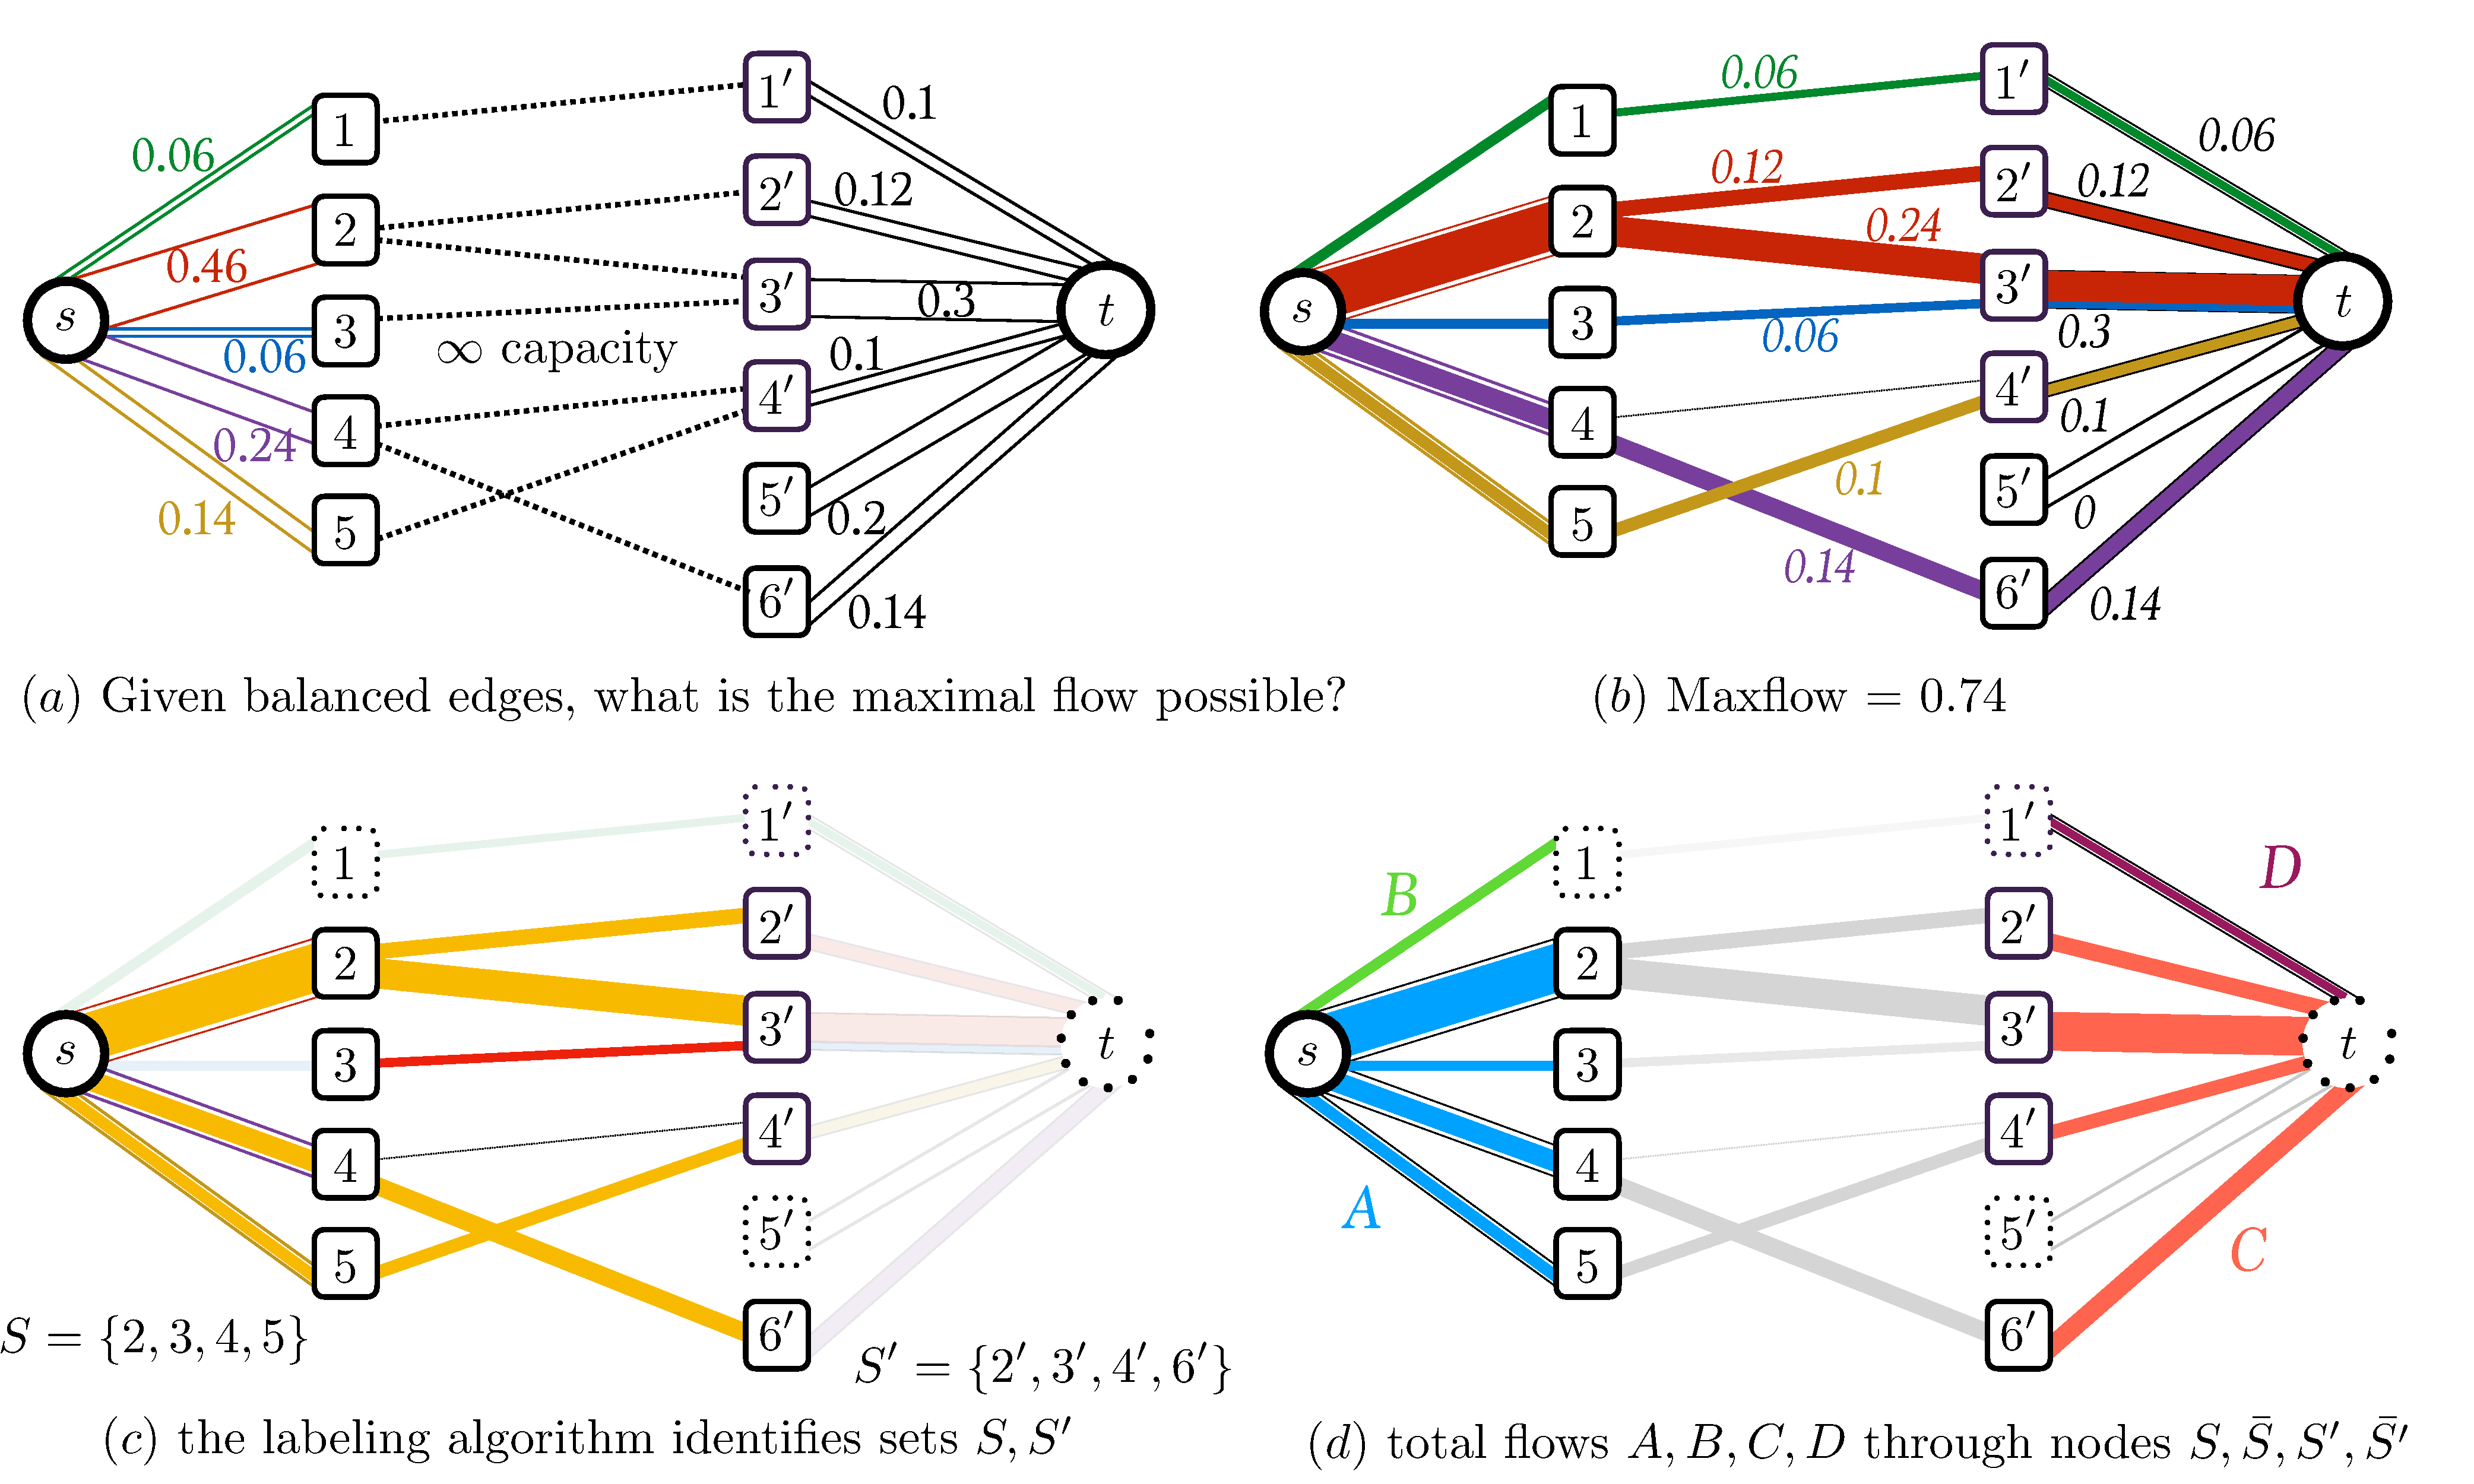
\includegraphics[width=\linewidth]{algo-basics-tree-solution/dual_ascent}
\caption{\label{fig-dualascent}
Consider a transportation problem involving the marginals introduced first in Figure~\ref{fig-f_of_P}, with $n=5, m=6$. Given two feasible dual vectors $\fD,\gD$, we try to obtain the ``best'' flow matrix $P$ that is complementary to $(\fD,\gD)$. Recall that this means that $\P$ can only take positive values on those edges $(i,j')$ corresponding to indices for which $\fD_i+\gD_j=\C_{i,j}$, here represented with dotted lines in plot (a). The best flow that can be achieved with that graph structure can be formulated as a max-flow problem in a capacitated network, starting from an abstract source node $s$ connected to all nodes labeled $i\in\range{n}$, terminating at an abstract terminal node $t$ connected to all nodes labeled $j'$, where $j\in\range{m'}$, and such that the capacities of edge $(s,i),(j',t), i\in \range{n},j\in\range{m}$ are respectively $\a_i,\b_j$ and all others infinite. The Ford--Fulkerson algorithm (\cite[p. 305]{bertsimas1997introduction}) can be applied to compute such a max-flow, which, as represented in plot (b), only achieves $0.74$ units of mass out of $1$ needed to solve the problem. One of the subroutines used by max-flow algorithms, the labeling algorithm (\cite[p. 308]{bertsimas1997introduction}), can be used to identify nodes that receive an unsaturated flow from $s$ (and recursively, all of its successors), denoted by orange lines in plot (c). The labeling algorithm also adds by default nodes that send a positive flow to any labeled node, which is the criterion used to select node $3$, which contributes with a red line to $3'$. Labeled nodes can be grouped in sets $S,S'$ to identify nodes which can be better exploited to obtain a higher flow, by modifying $\fD,\gD$ to obtain a different graph. The proof involves partial sums of flows described in plot (d)}
\end{figure}

The dual ascent method proceeds by modifying any feasible solution $(\fD,\gD)$ by any vector generated by sets $S,S'$ that ensure feasibility and improve the objective. When the sets $S,S'$ are those given by construction in the proof of Proposition~\ref{prop-dual-ascent-dir}, and the steplength $\varepsilon$ is defined as in the proof of Proposition~\ref{prop-feasibility-dual-pair}, we recover a method known as the \emph{primal-dual} method. That method reduces to the Hungarian algorithm for matching problems. Dual ascent methods share similarities with the dual variant of the network simplex, yet they differ in at least two important aspects. Simplex-type methods always ensure that the current solution is an \emph{extreme point} of the feasible set, $\PotentialsD(\C)$ for the dual, whereas dual ascent as presented here does not make such an assumption, and can freely produce iterates that lie in the interior of the feasible set. Additionally, whereas the dual network simplex would proceed by modifying $(\fD,\gD)$ to produce a primal solution $\P$ that satisfies linear (marginal constraints) but only nonnegativity upon convergence, dual ascent builds instead a primal solution $\P$ that is always nonnegative but which does not necessarily satisfy marginal constraints.

\section{Auction Algorithm}\label{s-auction}
The auction algorithm was originally proposed by~\citet{bertsekas1981new} and later refined in~\citep{bertsekas1988dual}. Several economic interpretations of this algorithm have been proposed (see \emph{e.g.} \citet{bertsekas1992auction}). The algorithm can be adapted for arbitrary marginals, but we present it here in its formulation to solve optimal assignment problems.

\paragraph{Complementary slackness.} Notice that in the optimal assignment problem, the primal-dual conditions presented for the optimal transport problem become easier to formulate, because any extremal solution $\P$ is \todoK{there always exist a permutation solution, but the converse it not true} necessarily a permutation matrix $\P_\si$ for a given $\si$ (see Equation~\eqref{prop-primal-dual-optimality}). Given primal $\P_{\si^\star}$ and dual $\fD^\star,\gD^\star$ optimal solutions we necessarily have that
$$
\fD^\star_i + \gD^\star_{\si^\star_i} = \C_{i,{\si_i^\star}}.
$$
Recall also that, because of the principle of $\C$-transforms enunciated in~\S\ref{sec-c-transforms}, that one can choose $\fD^\star$ to be equal to $\gD^{\bar\C}$. We therefore have that
\eql{\label{eq-dual-conditions-assign-1}
\C_{i,\si^\star_i} - \gD^\star_{\si_i}  = \min_{j} \C_{i,j} - \gD^\star_{j}. 
}
On the contrary, it is easy to show that if there exists a vector $\gD$ and a permutation $\sigma$ such that 
\eql{\label{eq-dual-conditions-assign}
\C_{i,\si_i} - \gD_{\si_i}  = \min_{j} \C_{i,j} - \gD_{j} 
}
holds, then they are both optimal, in the sense that $\si$ is an optimal assignment and $\gD^{\bar\C},\gD$ is an optimal dual pair. 


\paragraph{Partial assignments and $\varepsilon$-complementary slackness.} The goal of the auction algorithm is to modify iteratively a triplet $S,\xi,\gD$, where $S$ is a subset of $\range{n}$, $\xi$ a partial assignment vector, namely an injective map from $S$ to $\range{n}$, and $\gD$ a dual vector. The dual vector is meant to converge toward a solution satisfying an \emph{approximate} complementary slackness property~\eqref{eq-dual-conditions-assign}, whereas $S$ grows to cover $\range{n}$ as $\xi$ describes a permutation. The algorithm works by maintaining the three following properties after each iteration:
\begin{enumerate}[label={(\alph*)}]
	\item $\forall i\in S,\quad \C_{i,\xi_i} - \gD_{\xi_i}  \leq \varepsilon + \min_{j} \C_{i,j} - \gD_{j}$ ($\varepsilon$-CS).
	\item The size of $S$ can only increase at each iteration.
	\item There exists an index $i$ such that $\gD_i$ decreases by at least $\varepsilon$.
\end{enumerate}

\paragraph{Auction algorithm updates.} Given a point $j$ the auction algorithm uses not only the optimum appearing in the usual $\C$-transform but also a second best,
$$j^1_i \in \argmin_{j} \C_{i,j} - \gD_{j}, \quad j^2_i \in \argmin_{j\ne j^1_i} \C_{i,j} - \gD_{j}, $$
to define the following updates on $\gD$ for an index $i\notin S$, as well as on $S$ and $\xi$:
\begin{enumerate}\item \textbf{update $\gD$}: Remove to the $j^1_i$th entry of $\gD$ the sum of $\varepsilon$ and the difference between the second lowest and lowest adjusted cost $\{\C_{i,j}-\gD_j\}_j$,
\eql{
\begin{aligned}
	\gD_{j^1_{i}} &\leftarrow \gD_{j^1_{i}} - \underbrace{\left((\C_{i,j^2_{i}}-\gD_{j^2_{i}})-(\C_{i,j^1_{i}}-\gD_{j^1_{i}})+\varepsilon\right)}_{\geq \varepsilon >0}\label{eq-auction-update}\\
	&= \C_{i,j^1_{i}} - (\C_{i,j^2_{i}}-\gD_{j^2_{i}}) -\varepsilon.\\
\end{aligned}
}
\item \textbf{update $S$ and $\xi$}: If there exists an index $i'\in S$ such that $\xi_{i'}=j^1_{i}$, remove it by updating $S\leftarrow S\setminus \{i'\}$. Set $\xi_{i}=j^1_{i}$ and add $i$ to $S$, $S\leftarrow S \cup \{i\}.$
\end{enumerate}

\paragraph{Algorithmic properties.} The algorithm proceeds by starting from an empty set of assigned points $S=\emptyset$ with no assignment and empty partial assignment vector $\xi$, and $\gD=\zeros_n$, terminates when $S=\range{n}$, and loops through both steps above until it terminates. The fact that properties {(b)} and {(c)} are valid after each iteration is made obvious by the nature of the updates (it suffices to look at Equation~\eqref{eq-auction-update}). $\varepsilon$-complementary slackness is easy to satisfy at the first iteration since in that case $S=\emptyset$. The fact that iterations preserve that property is shown by the following proposition.
%Show::: $(\fD^{\,\tau})_i < (\fD^{\,\C\bar{\C}})_i$
\begin{prop} The auction algorithm maintains $\varepsilon$-complementary slackness at each iteration. 
\end{prop}
\begin{proof} 
	Let $\gD,\xi,S$ be the three variables at the beginning of a given iteration. We therefore assume that for any $i'\in S$ the relationship 
	$$\C_{i,\xi_{i'}} - \gD_{\xi_{i'}}  \leq \varepsilon + \min_{j} \C_{{i'},j} - \gD_{j} $$
holds. Consider now the particular $i\notin S$ considered in an iteration. Three updates happen: $\gD,\xi,S$ are updated to $\gD^{\text{n}},\xi^{\text{n}},S^{\text{n}}$ using indices $j^1_i$ and $j^2_i$. More precisely, $\gD^{\text{n}}$ is equal to $\gD$ except for element $j^1_i$, whose value is equal to
$$\gD_{j^1_{i}}^\text{n} = \gD_{j^1_{i}} - \left((\C_{i,j^2_{i}}-\gD_{j^2_{i}})-(\C_{i,j^1_{i}}-\gD_{j^1_{i}})\right)-\varepsilon \leq \gD_{j^1_{i}}-\varepsilon$$,
$\xi^{\text{n}}$ is equal to $\xi$ except for its $i$th element equal to $j^1_i$, and $S^{\text{n}}$ is equal to the union of $\{i\}$ with $S$ (with possibly one element removed). The update of $\gD^{\text{n}}$ can be rewritten
$$\gD^{\text{n}}_{j^1_i}= \C_{i,j^1_{i}} - (\C_{i,j^2_{i}}-\gD_{j^2_{i}}) -\varepsilon;$$
therefore we have
$$\C_{i,j^1_{i}} - \gD^{\text{n}}_{j^1_i}=  \varepsilon + (\C_{i,j^2_{i}}-\gD_{j^2_{i}}) = \varepsilon+\min_{j\ne j^1_i} (\C_{i,j}-\gD_{j}).$$
Since $-\gD\leq -\gD^{\text{n}}$ this implies that 
$$\C_{i,j^1_{i}} - \gD^{\text{n}}_{j^1_i} = \varepsilon + \min_{j\ne j^1_i} (\C_{i,j}-\gD_{j})\leq \varepsilon+\min_{j\ne j^1_i} (\C_{i,j}-\gD^{\text{n}}_{j}),$$
and since the inequality is also obviously true for $j=j^1_i$ we therefore obtain the $\varepsilon$-complementary slackness property for index $i$. For other indices $i'\ne i$, we have again that since $\gD^{\text{n}}\leq\gD$ the sequence of inequalities holds,
$$\C_{i,\xi^{\text{n}}_{i'}} - \gD^{\text{n}}_{\xi^{\text{n}}_{i'}} = \C_{i,\xi_{i'}} - \gD_{\xi_{i'}} \leq \varepsilon + \min_{j} \C_{{i'},j} - \gD_{j} \leq \varepsilon + \min_{j} \C_{{i'},j} - \gD^{n}_{j}. $$
\end{proof}

\begin{prop} The number of steps of the auction algorithm is at most $N=n\|\C\|_\infty/\varepsilon$.
\end{prop}
\begin{proof}Suppose that the algorithm has not stopped after $T>N$ steps. Then there exists an index $j$ which is not in the image of $\xi$, namely whose price coordinate $\gD_j$ has never been updated and is still $\gD_j=0$. In that case, there cannot exist an index $j'$ such that $\gD_{j'}$ was updated $n$ times with $n>\|\C\|_\infty/\varepsilon$. Indeed, if that were the case then for any index $i$
$$\gD_{j'}\leq-n\varepsilon<-\|\C\|_\infty\leq -\C_{i,j} = \gD_j-\C_{i,j},$$
which would result in, for all $i$,
$$\C_{i,j'}-\gD_{j'}> \C_{i,j}+ (\C_{i,j}-\gD_j),$$
which contradicts $\varepsilon$-CS. Therefore, since there cannot be more than $\|C\|_\infty/\varepsilon$ updates for each variable, the total number of iterations $T$ cannot be larger than $n\|\C\|_\infty/\varepsilon=N$.
\end{proof}

\begin{rem} Note that this result yields a naive number of operations of $N^3\|\C\|_\infty/\varepsilon$ for the algorithm to terminate. That complexity can be reduced to $N^3 \log\|\C\|_\infty$ when using a clever method known as $\varepsilon$-scaling, designed to decrease the value of $\varepsilon$ with each iteration (\cite[p. 264]{bertsekas1998network}).
\end{rem}

\begin{prop} The auction algorithm finds an assignment whose cost is $n\varepsilon$ suboptimal.
\end{prop}
\begin{proof}
	Let $\sigma,\gD^\star$ be the primal and dual optimal solutions of the assignment problem of matrix $\C$, with optimum $$t^\star=\sum \C_{i,\sigma_i} = \sum_i \min_{j}\C_{i,j}-\gD^\star_j+\sum_j\gD^\star_j.$$ 
Let $\xi,\gD$ be the solutions output by the auction algorithm upon termination. The $\varepsilon$-CS conditions yield that for any $i\in S$, 
$$\min_{j} \C_{i,j} - \gD_{j}\geq \C_{i,\xi_i} - \gD_{\xi_i} -\varepsilon.$$
Therefore by simple suboptimality of $\gD$ we first have
	$$\begin{aligned}t^\star&\geq \sum_i \left(\min_{j} \C_{i,j}-\gD_{j}\right) + \sum_j \gD_j\\
&\geq 
	\sum_i -\varepsilon+\left(\C_{i,\xi_i}-\gD_{\xi_i}\right) + \sum_j \gD_j = -n\varepsilon + \sum_i \C_{i,\xi_j} \geq  - n\varepsilon + t^\star.\end{aligned},$$
where the second inequality comes from $\varepsilon$-CS, the next equality by cancellation of the sum of terms in $\gD_{\xi_i}$ and $\gD_{j}$, and the last inequality by the suboptimality of $\xi$ as a permutation.	
\end{proof}


The auction algorithm can therefore be regarded as an alternative way to use the machinery of $\C$-transforms. Next we explore another approach grounded on regularization, the so-called Sinkhorn algorithm, which also bears similarities with the auction algorithm as discussed in~\citep{schmitzer2016stabilized}.
% $\fD^{\,\C\bar{\C}\C}\geq \fD^{\,\C}$ implies that $\fD^{\,\C\bar{\C}\C\bar{\C}}\leq \fD^{\,\C\bar{\C}}$
%

Note finally that, on low-dimensional regular grids in Euclidean space, it is possible to couple these classical linear solvers with multiscale strategies, to obtain a significant speed-up~\citep{schmitzer2016sparse,oberman2015efficient}.




%\section{Interior point methods}\label{s-ipm}
% \begin{rem}\label{rem:duality}Recall that a simple argument can help us recover the dual problem from the primal. For convenience, let us write $\q=\bigl[\begin{smallmatrix}\a\\ \b \end{smallmatrix} \bigr]$.
% 	Let $\U$ be the feasible set $\{\p\in\mathbb{R}^{nm}, \mathbf{A}\p = \q\}$.
% 	The feasible set's indicator function $\iota_\U$, such that $\iota_{\U}(\p)=0$ if $\p\in \U$ and $\infty$ otherwise,
% 	can be written as $\max_{\hD\in\mathbb{R}^{n+m}} -\hD^T(\mathbf{A}\p-\q)$.
% 	Indeed, the optimal value of that problem is obviously 0 when $\p$ is such that $\mathbf{A}\p=\q$, and $\infty$ otherwise, since it suffices to take for $\hD$ any negative constant that is large enough, and multiply it by vector $\mathbf{A}\p-\q$ to obtain an arbitrarily large objective value. Therefore, using the extended definition of convex functions, we have that
% $$\begin{aligned}
% \umin{\substack{\p \in \RR^{nm}_+\\\mathbf{A}\p = \q}} \cc^T\p & = \umin{\p \in \RR^{nm}_+} \cc^T\p + \iota_S(\p) =\umin{\p \in \RR^{nm}_+} \cc^T\p + \max_{\hD\in\mathbb{R}^{n+m}} -\hD^T(\mathbf{A}\p-\q)
% \\ & = \umin{\p \in \RR^{nm}_+}  \max_{\hD\in\mathbb{R}^{n+m}}  \cc^T\p - \hD^T(\mathbf{A}\p-\q)
% \\ & = \max_{\hD\in\mathbb{R}^{n+m}} \hD^T\q + \umin{\p \in \RR^{nm}_+} (\cc-\transp{\mathbf{A}}\hD)^T\p.
% \end{aligned}$$
% where we have assumed in the third line that one can inverse the orders of $\min$ and $\max$ problems. One can also notice that the term $\umin{\p \in \RR^{nm}_+} (\cc-\transp{\mathbf{A}}\hD)^T\p$ is minus the indicator function of the set $\R=\{\hD, \transp{\mathbf{A}}\hD\leq \cc\}$. Indeed, if any element of vector $\transp{\mathbf{A}}\hD$ is strictly bigger than $\cc$, say at index $i$, then the $i$-th element of $\cc-\transp{\mathbf{A}}\hD$ is negative, and it suffices to take for $\p$ the null vector except for its $i$-th index with an arbitrary large value to obtain and arbitrarily small value for the minimum. Therefore we have that
% $$
% \umin{\substack{\p \in \RR^{nm}_+\\\mathbf{A}\p = \q}} \cc^T\p = \max_{\hD\in\mathbb{R}^{n+m}} (\transp{\mathbf{A}}\hD)^T\q -\iota_{\R}(\hD)= \max_{\substack{\hD\in\mathbb{R}^{n+m}\\ \transp{\mathbf{A}}\hD\leq \cc}}\hD^T\q
% $$
% For a thorough and rigorous duality argument we refer the reader to~\cite[\S4.3]{bertsimas1997introduction}:
% \end{rem}

